\documentclass[a4paper]{tufte-handout}

\usepackage[portuguese]{babel}
\usepackage[T1]{fontenc}
\usepackage[utf8]{inputenc}
\usepackage{csquotes}

\newcommand{\workingDate}{\textsc{2024/2025}}
\newcommand{\userName}{João Sá Pereira}
\newcommand{\institution}{FEUP}

\usepackage{structure/lab_notes}
\newcommand{\graus}{$^{\circ}$C}

\newcommand{\TSP}{tiossulfato de sódio pentahidratado}
\newcommand{\tsp}{\ce{Na2S2O3.5H2O}}

\newcommand{\SCP}{sulfato de cobre pentahidratado}
\newcommand{\scp}{\ce{CuSO4.5H2O}}

\newcommand{\AMO}{amónia a 25~\%}
\newcommand{\amo}{\ce{NH3.H2O}}

\newcommand{\tioureia}{\ce{CH4N2S}}
\newcommand{\sulfe}{\ce{Fe2(SO4)3.5H2O}}
\newcommand{\acsul}{\ce{H2SO4}}

\newcommand{\bromo}{\ce{NaBr}}
\newcommand{\acl}{\ce{HCl}}
\newcommand{\hipso}{\ce{NaOCl}}

\newcommand{\sulfcu}{\ce{CuSO4.5H2O}}
\newcommand{\hidso}{\ce{NaOH}}
\newcommand{\citratodi}{\ce{C6H7NaO7}}

\newcommand{\bromopot}{\ce{KBrO3}}
\newcommand{\cloretofe}{\ce{FeCl3}}

%%%%%%%%%%%%%%% TITLE page %%%%%%%%%%%%%%%
\title{Notas de Laboratório}
\subtitle{Bolsa de Investigação - INN4MIN}
\author[João Sá Pereira]{João Sá Pereira}
\date{2024/2025}
\publisher{Faculdade de Engenharia da Universidade do Porto}

\begin{document}

\selectlanguage{portuguese}
%%%%%%%%%%%%%%% TITLE %%%%%%%%%%%%%%%
\maketitlepage
\newpage
\thispagestyle{empty}
	\topskip0pt
	\vspace*{\fill}
	\begin{projects}
		\begin{description}
			\item [INN4MIN] Desenvolvimento de metodologias inovadoras e sustentáveis aplicadas a recuperação de ouro e elementos críticos em minérios e placas de circuito integradas utilizadas\footnote{\href{https://cerena.pt/projects/inn4min-development-innovative-and-sustainable-approaches-applied-recovery-gold-and-1}{ERA-MIN3/0003/2021}}
		\end{description}
	\end{projects}

	\begin{planos}
		Lixiviação de uma amostra de ouro da mina do Numão (pré-concentrado, cerca de 15~kg)
		\begin{description}
			\item [Preparação de amostras:] Amostragens para sacos de 200/250~g.
			\item [Caracterização de amostras:] FRX, Digestão ABS, análise granulométrica $\rightarrow$ fazer em triplicado.
			\item [Lixiviação:] Plano de lixiviação com Tioreia (fazer exploratório e depois preparar plano de ensaios)
			\item [Lixiviação:] Plano de lixiviação com Citrato.
			\item [Lixiviação:] Plano de lixiviação com Bromo.
		\end{description}
		Fazer ensaios exploratórios com os 3 reagentes e, em função dos resultados, preparar plano mais exaustivo.
	\end{planos}

	\vspace*{\fill}
\newpage

%%%%%%%%%%%% Beggining of document %%%%%%%%%%%%%%%%%%%%%%
%%%%%%%%%%%%%%%%%%%%%%%%%%%%%%%%%%%%%%%%%%%%%%%%%%%%%%%%
\pagestyle{fancy}
% \thispagestyle{empty}
\topskip0pt
\vspace*{\fill}
\begin{fullwidth}
    \centering
    \LARGE{\textbf{Parte I: Preparação e Caracterização de Amostras}}
\end{fullwidth}
\vspace*{\fill}
% \newpage
% \section*{Preparação e Caracterização de Amostras}

\newday{21 Outubro 2024}

Foi feito um trabalho de desagregação da amostra inicial, proveniente da mina do Numão.
Uma amostra de um pré-concentrado que tinha sido anteriormente submetida a processos de flutuação.
A amostra tinha cerca de 15~kg.

\begin{marginfigure}
    \includegraphics[width=\linewidth]{figures/moinho_tm300}
    \caption{Moinho de tambor \href{https://www.retsch.pt/pt/produtos/trituracao/moinhos-planetarios-e-de-bolas/tm-300/}{TM 300 Retsch}.}
    \label{fig:moinho_tm300}
\end{marginfigure}

Foi utilizado um moinho de bolas - apresentado na Figura~\ref{fig:moinho_tm300} - com a seguinte configuração de trabalho:
\begin{itemize}
    \item[-] 60 rpm;
    \item[-] Duração de trabalho 30~minutos;
\marginnote{Como o moinho nunca tinha sido utilizado para desagregar amostras, fez-se testes para determinar o tempo necessário de funcionamento e para determinar também a necessidade ou não de bolas.}
    \item[-] Sentido de rotação inverte de 5 em 5~minutos;
    \item[-] Pausa de 1~minuto entre cada inversão de sentido;
    \item[-] 3,41~kg de bolas.
\end{itemize}

Foi-se colocando partes da amostra dentro do tambor do moinho e deixou-se a desagregar durante o tempo estipulado.
\marginnote{O peneiro de \#1.18~mm foi utilizado como redundância, apenas para ter a certeza que toda a amostra estava desagregada.}
Uma vez terminado o tempo de funcionamento do moinho, peneirou-se o material desagregado com um peneiro de malha \#1.18~mm.
Foi-se fazendo este procedimento sucessivamente.
Deixou-se material para o dia seguinte.

\hrulefill

%%%%%%%%%%%%%%%%%%%%%%%%%%%%%%%%%%%%%%%%%%%%%%%%%%%%%%%%

\newday{22 Outubro 2024}

\textit{Na Figura~\ref{fig:amostra_no_moinho} temos a amostra de material dentro do tambor do moinho.}

\begin{marginfigure}[4\baselineskip]
    \includegraphics[width=0.9\linewidth]{figures/amostra_no_moinho}
    \caption{Amostra de material no tambor do moinho.}
    \label{fig:amostra_no_moinho}
\end{marginfigure}

Do dia anterior verificou-se que ainda havia alguns ``blocos'', portanto meteu-se o moinho a trabalhar durante cerca de 15~minutos para desagregar o resto do material.
Quando este terminou, a totalidade da amostra foi desagregada e peneirada com o peneiro \#1.18~mm.

Com o material já desagregado, era necessário agora homogeneizar a amostra.
Para isso, foi utilizado o separador \emph{Jones}\sidenote{O separador \emph{Jones}, ou em inglês \emph{riffle splitter}, é utilizado para separar amostras em duas partes quase idênticas.} (esquartelador).
Separou-se a amostra de $\approx$~15~kg em duas amostras de $\approx$~7,5~kg cada - amostra \texttt{A} e amostra \texttt{B}\@.

A amostra B vai ser guardada.
Foi armazenada em dois sacos de plástico - \texttt{B1} = 3,36~kg e \texttt{B2} = 4,28~kg.
A amostra \texttt{A} será posteriormente separada em sacos de $\approx$~1~kg.

\hrulefill
\pagebreak
%%%%%%%%%%%%%%%%%%%%%%%%%%%%%%%%%%%%%%%%%%%%%%%%%%%%%%%%

\newday{24 Outubro 2024}

\textit{N.B.: Antes de se utilizar o separador \emph{Jones}, tinha sido feita uma separação manual. Esta abordagem não poderia estar mais errada, separar a amostra manualmente introduz erros significativos, especialmente em amostras com partículas de diferentes calibres. O Jones é uma das formas representativas e precisas de separação de amostras e é o que será utilizado neste trabalho.}

\marginnote{É importante ter em consideração que obtêm-se sempre duas amostras com o separador \textit{Jones}, mas que uma das metades obtidas é \textbf{sempre} descartada. Ou seja, na Figura~\ref{fig:diagrama_jones}, o ramo da direita de cada uma das ramificações foi descartado para ser separado posteriormente (a totalidade da amostra foi separada em sacos de $\approx$~1~kg).}

\subsection{Funcionamento do separador Jones}\label{subsec:funcionamento-do-separador-jones}

O \emph{Jones} separa uma amostra em duas metades, sendo que uma das metades separadas é descartada e trabalha-se com a outra.

Um esquema de funcionamento desta separação está apresentado na Figura~\ref{fig:diagrama_jones}.

\begin{figure}[!ht]
    \centering
    \includegraphics[width=0.9\textwidth]{figures/diagrama_jones}
    \caption{Diagrama de separação de amostras com o Jones.}
    \label{fig:diagrama_jones}
\end{figure}

A amostra foi separada, com o separador \textit{Jones}, em sacos de aproximadamente 1~kg.
A massa de cada saco está apresentada na Tabela~\ref{tab:massa_sacos}.

\begin{table}[!htbp]
    \centering
    \begin{tabularx}{\textwidth}{@{}lC@{}}
        \toprule
        \textbf{Amostra} & \textbf{Massa (g)} \\ \midrule
        \textcolor{customblue}{A$_{01}$} & \textcolor{customblue}{1020,66} \\
        A$_{02}$ & 836,56 \\
        A$_{03}$ & 802,66 \\
        \textcolor{customorange}{A$_{04}$} & \textcolor{customorange}{1052,15} \\
        A$_{05}$ & 986,89 \\
        A$_{06}$ & 786,81 \\
        A$_{07}$ & 1138,15 \\
        \textcolor{customgreen}{A$_{08}$} & \textcolor{customgreen}{1044,50} \\ \midrule
        \textbf{Total} & 7590,38 \\ \bottomrule
    \end{tabularx}
    \caption{Massa dos amostras separadas com o \emph{Jones}.}
    \label{tab:massa_sacos}
\end{table}

\marginnote[-0.5cm]{As células destacadas representam as amostras escolhidas para crivagem, que vai ser realizada posteriormente.}

\hrulefill

%%%%%%%%%%%%%%%%%%%%%%%%%%%%%%%%%%%%%%%%%%%%%%%%%%%%%%%%
\pagebreak

\newday{28 Outubro 2024}

Hoje foi realizada a crivagem do material previamente separado.
Escolheu-se, aleatoriamente, três dos oito sacos.
Os sacos escolhidos para crivagem foram os seguintes: \texttt{A01}, \texttt{A04} e \texttt{A08}; destacados na Tabela~\ref{tab:massa_sacos}.

A série de crivos utilizada para crivagem foi a seguinte:

\begin{minipage}{0.4\textwidth}
    \begin{enumerate}
        \item 0,850~mm
        \item 0,600~mm
    \end{enumerate}
\end{minipage}
\begin{minipage}{0.4\textwidth}
    \begin{enumerate}
        \setcounter{enumi}{2}
        \item 0,425~mm
        \item 0,300~mm
    \end{enumerate}
\end{minipage}

O material foi crivado nos crivos mecânicos\sidenote{Uma particularidade dos crivos mecânicos utilizados é que estes tinham a funcionalidade de definir automaticamente a frequência de vibração de acordo com o peso da coluna de crivos.} durante 30~minutos.
A mesma série de crivos foi utilizada para os três sacos.

Após cada crivagem, a massa das frações de material retido em cada um dos crivos da série de crivagem foi medida e está apresentada na Tabela~\ref{tab:massa_retido_crivagem}:

\begin{table}[!htb]
    \centering
    \begin{tabularx}{\textwidth}{@{}lCCC@{}}
        \toprule
        \multirow{2}{*}{\textbf{Malha (mm)}} & \multicolumn{3}{c}{\textbf{Massa (g)}} \\ \cmidrule(lr){2-4}
         & \multicolumn{1}{C}{\textbf{A$\bm{_{01}}$}} & \multicolumn{1}{C}{\textbf{A$\bm{_{04}}$}} & \textbf{A$\bm{_{08}}$} \\ \hline
        \textbf{0,850} & \multicolumn{1}{C}{4,72} & \multicolumn{1}{C}{4,82} & 4,69 \\
        \textbf{0,600} & \multicolumn{1}{C}{4,26} & \multicolumn{1}{C}{4,48} & 4,43 \\
        \textbf{0,425} & \multicolumn{1}{C}{7,06} & \multicolumn{1}{C}{8,15} & 9,65 \\
        \textbf{0,300} & \multicolumn{1}{C}{30,65} & \multicolumn{1}{C}{31,53} & 41,93 \\
        \textbf{Infra} & \multicolumn{1}{C}{973,37} & \multicolumn{1}{C}{1002,44} & 982,95 \\ \midrule
        \textbf{\bm{$\sum$}}& \multicolumn{1}{C}{\textbf{1020,06}} & \multicolumn{1}{C}{\textbf{1051,42}} & \textbf{1043,65} \\ \bottomrule
    \end{tabularx}
    \caption{Massa de material retido em cada crivo após a crivagem.}
    \label{tab:massa_retido_crivagem}
\end{table}

Foi efetuada uma análise granulométrica do material retido em cada crivo.
A curva granulométrica está apresentada na Figura~\ref{fig:curva_granulometrica}.

\begin{figure}[!htb]
    \centering
    \begin{tikzpicture}[font=\footnotesize]
    \begin{axis}[
        title={Curva Granulométrica},
        xlabel={Crivo (mm)},
        ylabel={Cumulante Inferior (\%)},
        xmode=log,
        xtick={0.1, 1, 10},
        xticklabel style={/pgf/number format/fixed},
        log ticks with fixed point,
        xmin=0.1, xmax=10,
        ymin=93, ymax=100,
        ylabel near ticks,
        yticklabel=\pgfmathprintnumber{\tick},
        width=10cm,
        height=8cm,
        grid=both,
        grid style={dashed, gray!30},
        enlarge x limits={abs=0.5cm},
        axis lines= left,
        legend pos=south east,
        height=6.5cm,
    ]
    % Série A01
    \addplot[
        mark=*,
        mark options={scale=1, fill=customblue},
        color=customblue,
        line width=0.7pt
    ] coordinates {
        (1.18, 100.00)
        (0.850, 99.54)
        (0.600, 99.12)
        (0.425, 98.43)
        (0.300, 95.42)
    };
    \addlegendentry{A01}

    % Série A04
    \addplot [
        mark=*,
        mark options={scale=1, fill=customorange},
        color=customorange,
        line width=0.7pt
    ] coordinates {
        (1.18, 100.00)
        (0.850, 99.54)
        (0.600, 99.12)
        (0.425, 98.34)
        (0.300, 95.34)
    };
    \addlegendentry{A04}

    % Série A08
    \addplot[
        mark=*,
        mark options={scale=1, fill=customgreen},
        color=customgreen,
        line width=0.7pt
    ]  coordinates {
        (1.18, 100.00)
        (0.850, 99.55)
        (0.600, 99.13)
        (0.425, 98.20)
        (0.300, 94.18)
    };
    \addlegendentry{A08}

    \end{axis}
    \end{tikzpicture}
    \caption{Curva granulométrica.}
    \label{fig:curva_granulometrica}
\end{figure}

Como existe muito pouco material acima do calibre 0,300~mm (<~5~\%), juntou-se todas as frações de material novamente e vai-se realizar medições no granulómetro laser.

\hrulefill
\pagebreak
%%%%%%%%%%%%%%%%%%%%%%%%%%%%%%%%%%%%%%%%%%%%%%%%%%%%%%%%

\newday{30 Outubro 2024}

\newthought{Granulómetro Laser} \href{https://www.malvernpanalytical.com/en/support/product-support/mastersizer-range/mastersizer-2000}{Malvern Mastersizer 2000}

\marginnote{Um granulómetro laser utiliza a difração da luz laser para medir a distribuição dos tamanhos das partículas numa amostra. Este tipo de análise é particularmente útil porque permite uma análise rápida, precisa e repetível.}

Continuando o trabalho, as frações das amostras previamente crivadas foram colocadas todas na sua forma original (amostra tal-qual de $\approx$~1~kg) para se analisar a granulometria dos 8~sacos de material, com auxílio do granulómetro laser - Figura~\ref{fig:granulometro_laser}.

\begin{figure}[!htb]
    \centering
    \includegraphics[width=0.75\linewidth]{figures/granulometro_laser}
    \caption{Granulómetro laser Malvern Mastersizer 2000.}
    \label{fig:granulometro_laser}
\end{figure}

Começou-se por analisar a amostra \texttt{A01}\sidenote[][-0.25cm]{As amostras foram analisadas separadamente, mas com os resultados obtidos de todas as subamostras poderemos generalizar para a amostra tal-qual ($\approx$~15~kg).}.
A primeira análise foi feita com a amostra seca (ou seja, foi colocada no granulómetro sem estar misturada em água), de forma a avaliar a distribuição do tamanho das partículas.
Verificou-se que havia partículas ainda agregadas\sidenote{Como estamos a trabalhar com material de calibre muito fino, é normal haver agregação de partículas. Isto pode ser combatido com uma agitação forte; uso de ultra-som ou mistura prévia em água para desagregar.}.

Limpou-se o granulómetro e fez-se outra análise desta vez tendo misturado a amostra em água para evitar a agregação das partículas.
Mesmo assim, era possível melhorar ainda mais os resultados e portanto utilizou-se a opção de ultra-som para promover ainda mais a desagregação das partículas.

Visto que com uma mistura prévia em água e com a utilização da opção de ultra-som do granulómetro obtiam-se os melhores resultados, os restantes sacos foram analisados com estas parametrizações.
Sendo que, antes de se ativar o ultra-som\sidenote{A utilização do ultra-som, se for possível, deve ser evitada pois como as partículas são muito finas pode promover a fragmentação e resultar em análises erradas que não refletem a verdadeira composição da amostra.} realizou-se sempre uma análise apenas com a mistura prévia em água.

As análises foram identificadas da seguinte forma:
\begin{itemize}
    \item[-] \texttt{A0n}, sendo \texttt{n} o número da amostra, para análises sem mistura prévia em água e sem ultra-som;
    \item[-] \texttt{A0n-REP}, para análise com mistura prévia em água e sem ultra-som;
    \item[-] \texttt{A0n-REP2}, para análise com mistura prévia em água e com ultra-som.
\end{itemize}

\marginnote[-0.5cm]{Para cada análise foram guardados ficheiros distintos com uma curva granulométrica e com uma curva de distribuição de calibres, \texttt{A0n-REP2-CUM} e \texttt{A0n-REP2-FREQ}, respetivamente.}

Os dados das análises foram guardados para uso posterior.

\hrulefill
\pagebreak

%%%%%%%%%%%%%%%%%%%%%%%%%%%%%%%%%%%%%%%%%%%%%%%%%%%%%%%%

\newday{31 Outubro 2024}\label{day:31-outubro-2024}

\begin{marginfigure}[3\baselineskip]
    \centering
    \includegraphics[width=0.55\linewidth]{figures/divisor_de_amostras_retsch}
    \caption{Divisor de amostras \href{https://www.retsch.pt/pt/produtos/assistencia/amostradores/pt-100/}{PT 100}.}
    \label{fig:divisor_de_amostras_retsch}
\end{marginfigure}

Uma fez realizada a análise granulométrica no granulómetro laser, iremos dar continuação à amostragem.
O próximo passo será dividir as amostras de 1~kg em sub-amostras de, aproximadamente 0,250~g - deveremos ter no máximo 250~g e no mínimo 200~g.

Para esta divisão foi utilizado o divisor de amostras apresentado na Figura~\ref{fig:divisor_de_amostras_retsch}.
Este equipamento em específico, divide a amostra em 8~partes iguais.
Portanto, das nossas amostras de $\approx$~1~kg iremos obter 8 sub-amostras de $\approx$~0,125~kg.
Como queremos que as nossas sub-amostras tenham $\approx$~0,250~kg, iremos juntar os frascos resultantes da divisão 2~a~2.

O funcionamento do divisor de amostras é bastante simples e direto.
Coloca-se os frascos, liga-se o equipamento, liga-se o alimentador e coloca-se a amostra (pouco a pouco para prevenir entupimentos) no funil do alimentador\sidenote{O divisor de amostras conta com o alimentador \href{https://www.retsch.pt/pt/produtos/assistencia/alimentadores/}{DR 100} que promove a alimentação contínua de material ao divisor.}.
O divisor faz o resto do trabalho, dividindo a amostra em 8~sub-amostras praticamente iguais.

Das 8~sub-amostras obtidas em cada uma das divisões, constitui-se sacos de $\approx$~0,250~kg, juntando os frascos 2~a~2.
As massas de cada uma das sub-amostras está apresentada na tabela seguinte:

\begin{table*}[ht]
\centering
    \begin{tabularx}{\textwidth}{@{}lCCCCCCCC@{}}
        \toprule
        \textbf{Amostra} & \textbf{A\bm{$_{01}$} (g)} & \textbf{A\bm{$_{02}$} (g)} & \textbf{A\bm{$_{03}$} (g)} & \textbf{A\bm{$_{04}$} (g)} & \textbf{A\bm{$_{05}$} (g)} & \textbf{A\bm{$_{06}$} (g)} & \textbf{A\bm{$_{07}$} (g)} & \textbf{A\bm{$_{08}$} (g)} \\ \hline
        \textbf{A\bm{$_{0\text{n.}1}$}} & 254,44 & 207,90 & 200,00 & 262,99 & 243,20 & 196,06 & 283,14 & 264,14 \\
        \textbf{A\bm{$_{0\text{n.}2}$}} & 253,67 & 208,76 & 202,18 & 262,30 & 245,76 & 192,84 & 286,50 & 260,05 \\
        \textbf{A\bm{$_{0\text{n.}3}$}} & 254,76 & 210,29 & 200,52 & 262,23 & 250,16 & 198,40 & 284,01 & 257,18 \\
        \textbf{A\bm{$_{0\text{n.}4}$}} & 254,22 & 209,50 & 198,21 & 262,28 & 246,06 & 198,43 & 282,14 & 259,72 \\ \midrule
        \textbf{\bm{$\sum$}} & 1017,09 & 836,45 & 800,91 & 1049,80 & 985,18 & 785,73 & 1135,79 & 1041,09 \\ \bottomrule
    \end{tabularx}
\end{table*}

\newpara

Uma vez divididas as sub-amostras, iremos escolher um dos sacos de $\approx$~250~g proveniente da divisão de cada um dos 8 sacos de $\approx$~1~kg.
Estas 8 sub-amostras irão ser analisadas no FRX\sidenote{A fluorescência de raios X (FRX) é uma técnica rápida e não destrutiva amplamente usada para determinar a composição elementar de um material que requer apenas uma preparação mínima da amostra.} para determinar a composição química das amostras.
Como o teor em \ce{Au} deve ser muito pequeno, ele não será determinado por esta análise, obteremos apenas os elementos em maior quantidade.

Foram escolhidas as amostras \texttt{A01.1}, \texttt{A02.3}, \texttt{A03.2}, \texttt{A04.3}, \texttt{A05.3}, \texttt{A06.4}, \texttt{A07.4} e \texttt{A08.3} para serem analisadas no FRX\@.

\begin{marginfigure}[1\baselineskip]
    \centering
    \includegraphics[width=0.7\linewidth]{figures/FRX}
    \caption{Equipamento FRX utilizado.}
    \label{fig:equipamento_frx}
\end{marginfigure}

O funcionamento do equipamento FRX é bastante simples, basta colocar a amostra dentro do equipamento, fechar bem a porta e acionar o gatilho para começar a análise.
Foram realizados cinco ``tiros'' por amostra, com um tempo de análise de 30~segundos em cada tiro.
No fim de cada tiro, foi-se alterando a posição da amostra dentro do equipamento, para que fossem analisadas diferentes partes da amostra de forma a que os resultados sejam representativos.

Os resultados das análises foram descarregados em formato \texttt{.csv}.
Os dados irão ser posteriormente analisados.

%%%%%%%%%%%%%%%%%%%%%%%%%%%%%%%%%%%%%%%%%%%%%%%%%%%%%%%%

\newday{6 Novembro 2024}\label{day:6-novembro-2024}

Hoje foram refeitas as análises FRX para as amostras \texttt{A01.1}, \texttt{A03.2}, \texttt{A05.3} e \texttt{A08.3}.
Os valores destas análises serão adicionados (substituídos) aos dados obtidos no dia~\nameref{day:31-outubro-2024}.

A necessidade de refazer as análises para estas amostras assenta no facto de o equipamento não ter feito leituras de alguns elementos em alguns dos 5~tiros realizados.
Portanto, é necessário refazer a análise FRX para estas amostras para que a média, que vai ser calculada, seja correta e que os resultados sejam representativos.

\hrulefill

\subsection*{Análise dos resultados do FRX}

Das análises realizadas, tanto a primeira, do dia~\nameref{day:31-outubro-2024}, como a segunda, do dia~\nameref{day:6-novembro-2024}, foram obtidos ficheiros \texttt{.csv} que continham informação relativa à quantidade (em \%) de elementos presentes em cada uma das amostras.

Uma análise foi realizada aos valores obtidos a partir desses ficheiros.
Para cada tiro e para cada elemento, identificaram-se e excluíram-se os valores considerados \emph{outliers}\sidenote{Por exemplo, em alguns tiros, certos elementos tinham quatro valores a rondar os 2~\% e um valor a rondar os 0,002~\%. Nesses casos, o outlier seria o 0,002~\%, que não se comporta como os restantes valores para a mesma amostra.}, ou seja, aqueles que apresentavam um desvio significativo em relação aos restantes.
Essa exclusão permitiu que a média calculada fosse mais representativa das características de cada amostra.

Como resultado dessa análise, foi elaborada a Tabela~\ref{tab:frx-elementos-mais-presentes}, que apresenta os valores médios das quantidades dos elementos (em \%), organizados em ordem decrescente para cada uma das amostras.
Apenas os elementos com maior presença foram incluídos:

\begin{table}[!ht]
    \caption{FRX - Elementos mais presentes nas amostras.}
    \label{tab:frx-elementos-mais-presentes}
    \begin{tabularx}{\textwidth}{@{}lCCCCCCCC@{}}
        \toprule
        \textbf{(\%)} & \textbf{A01.1} & \textbf{A02.3} & \textbf{A03.2} & \textbf{A04.3} & \textbf{A05.3} & \textbf{A06.4} & \textbf{A07.4} & \textbf{A08.3} \\ \midrule
        \textbf{Fe} & 4,582 & 4,977 & 4,480 & 4,871 & 4,608 & 4,268 & 4,665 & 4,341 \\
        \textbf{As} & 1,916 & 2,052 & 1,844 & 2,048 & 1,908 & 1,718 & 1,947 & 1,777 \\
        \textbf{K} & 1,531 & 1,721 & 1,331 & 1,629 & 1,416 & 1,504 & 1,947 & 1,833 \\
        \textbf{Ti} & 0,211 & 0,263 & 0,226 & 0,247 & 0,251 & 0,225 & 0,270 & 0,232 \\ \bottomrule
    \end{tabularx}
\end{table}

\newpara

Com esta tabela, de forma a ser possível visualizar os dados obtidos graficamente, construiu-se um gráfico de barras com os elementos mais presentes, \ce{Fe}, \ce{As}, \ce{K} e \ce{Ti}, apresentada na Figura~\ref{fig:frx-elementos-mais-presentes}.

Os restantes elementos não serão aqui apresentados pois estão presentes numa quantidade muito pequena.
Os dados referentes aos restantes elementos podem ser consultados na pasta partilhada do projeto.

\newpage

\begin{figure}[!htb]
    \centering
    \begin{tikzpicture}[font=\footnotesize]
    \centering
      \begin{axis}[
            ybar, axis on top,
            title={Elementos mais presentes nas amostras},
            height=7cm, width=11cm,
            bar width=0.175cm, % Reduzi o tamanho das barras
            axis lines=left,
            x axis line style={opacity=0},
            ymin=0, ymax=6,
            enlarge x limits=true, % Espaçamento proporcional entre os grupos
            ylabel={\% Elemento},
            ytick = {0,1,2,3,4,5,6},
            yticklabel={\pgfmathprintnumber{\tick}~\%},
            symbolic x coords={A01.1, A02.3, A03.2, A04.3, A05.3, A06.4, A07.4, A08.3},
            xtick=data,
            legend style={
                at={(0.5,-0.15)},
                anchor=north,
                legend columns=-1,
                /tikz/every even column/.append style={column sep=0.5cm}
            },
            % Adicionar rótulos às barras (rotacionados para melhor espaçamento)
            nodes near coords,
            every node near coord/.append style={
                font=\scriptsize, rotate=90, anchor=west
            }
        ]

        % Adicionando as barras
        \addplot+[draw=none, color=customblue]
            coordinates {(A01.1,4.5818) (A02.3,4.9766) (A03.2,4.4801) (A04.3,4.8707) (A05.3,4.6077) (A06.4,4.2681) (A07.4,4.6648) (A08.3,4.3410)};
        \addlegendentry{Fe};

        \addplot+[draw=none, color=customorange]
            coordinates {(A01.1,1.9157) (A02.3,2.0522) (A03.2,1.8442) (A04.3,2.0483) (A05.3,1.9080) (A06.4,1.7179) (A07.4,1.9466) (A08.3,1.7770)};
        \addlegendentry{As};

        \addplot+[draw=none, color=customcinza]
            coordinates {(A01.1,1.5312) (A02.3,1.7211) (A03.2,1.3313) (A04.3,1.6292) (A05.3,1.4163) (A06.4,1.5042) (A07.4,1.9466) (A08.3,1.8327)};
        \addlegendentry{K};

        \addplot+[draw=none, color=customyellow]
            coordinates {(A01.1,0.2109) (A02.3,0.2631) (A03.2,0.2261) (A04.3,0.2470) (A05.3,0.2508) (A06.4,0.2246) (A07.4,0.2695) (A08.3,0.2317)};
        \addlegendentry{Ti};

      \end{axis}
    \end{tikzpicture}
    \caption{FRX - Elementos mais presentes nas amostras.}
    \label{fig:frx-elementos-mais-presentes}
\end{figure}

\hrulefill

%%%%%%%%%%%%%%%%%%%%%%%%%%%%%%%%%%%%%%%%%%%%%%%%%%%%%%%%

\newday{7 Novembro 2024}\label{day:7-novembro-2024}

Hoje foi feita a preparação para fazer a digestão ácida\sidenote{A digestão ácida serve para decompor a matriz mineral da amostra, permitindo a solubilização dos elementos de interesse (neste caso, o ouro e possivelmente outros metais associados) e eliminando interferências que poderiam afetar a análise subsequente por espectrometria de absorção atómica.}.
Para isso foi escolhida, aleatoriamente, uma sub-amostra de $\approx$~250~g para este procedimento.
Foi escolhida a amostra \texttt{A08.3}, com 257,18~g.

Como vão ser necessários apenas 50~g de amostra, a \texttt{A08.3} foi colocada no divisor de amostras - o mesmo da Figura~\ref{fig:divisor_de_amostras_retsch}.

Do divisor de amostras obteu-se 54,15~g (\texttt{A08.3.1}) que foi depois dividido em cinco copos, cada um com aproximadamente 10~g.
Estes cinco copos foram depois colocados na mufla.
A mufla foi programada para aquecer até 700~\graus, manter os 700~\graus \, durante 1~hora e depois desligar-se automaticamente.
As amostras ficam a arrefecer dentro da mufla até ao dia seguinte.
\begin{marginfigure}[1\baselineskip]
    \centering
    \includegraphics[width=0.7\textwidth]{figures/Mufla}
    \caption{Mufla utilizada para aquecer a amostra.}
    \label{fig:mufla}
\end{marginfigure}

A amostra \texttt{A08.3} foi reconstituída com o material que não foi para os copos da mufla e foi medida a massa: 215.03~g (com o peso do saco).

No dia seguinte, com a amostra já arrefecida, será realizada a digestão ácida, sendo que o procedimento será posteriormente explicado.

\hrulefill

%%%%%%%%%%%%%%%%%%%%%%%%%%%%%%%%%%%%%%%%%%%%%%%%%%%%%%%%

\newday{8 Novembro 2024}\label{day:8-novembro-2024}

Retiraram-se as amostras que foram colocadas na mufla no dia~\nameref{day:7-novembro-2024}.
O material, anteriormente com uma cor beje (como se pode ver na Figura~\ref{fig:amostra_no_moinho}), encontra-se agora com uma cor avermelhada - Figura~\ref{fig:amostra-apos-mufla}.

\begin{marginfigure}[0.25cm]
    \centering
    \includegraphics[width=0.9\linewidth]{figures/Amostra após mufla}
    \caption{Amostra após a mufla.}
    \label{fig:amostra-apos-mufla}
\end{marginfigure}

O material foi transferido para gobelés brancos para serem submetidos à digestão ácida.
A digestão será feita com ácido nítrico, \ce{HNO_3}; e com ácido clorídrico, \ce{HCl}.
A relação vai ser de 1:3, ou seja, 6~ml de \ce{HNO_3} para 18~ml de \ce{HCl}, a 200~\graus.

A quantidade específicada de cada ácido é colocada em cada um dos 5~copos da Figura~\ref{fig:amostra-a-ser-atacada}, deixando a reação decorrer durante 1~hora e 30~minutos.
Serão feitos 3~ataques, ou seja, após cada hora e meia será colocado de novo ácido nítrico e ácido clorídrico.
Repete-se esta operação três vezes, totalizando em 4~horas e 30~minutos de reação.

\begin{marginfigure}[2\baselineskip]
    \centering
    \includegraphics[width=0.9\linewidth]{figures/Amostra a ser atacada - digestão ácida}
    \caption{Amostra a ser atacada com \emph{aqua regia}.}
    \label{fig:amostra-a-ser-atacada}
\end{marginfigure}

Após o terceiro e último ataque, foram adicionados 4~ml de \ce{HCl} a cada um os copos.
É necessário agora transferir o material dissolvido e separá-lo dos resíduos.
Para isso, com o auxílio de uma pinça, retirou-se o copo da areia, agitou-se um pouco o líquido no interior e transferiu-se cuidadosamente para um balão volumétrico de 50~ml tendo cuidado para parar de verter quando a cor do líquido passar de laranja para um verde acinzentado (o material verde acinzentado é o resíduo).
O restante volume do balão volumétrico foi preenchido com água destilada.

O resíduo foi colocado numa placa de Petri.
Colocou-se um pouco de água destilada no copo para facilitar a transferência do resíduo para a placa.
Fez-se isto para cada um dos 5~copos, resultando nas amostras apresentadas na Figura~\ref{fig:amostra-apos-digestao}.

\begin{marginfigure}[-1\baselineskip]
    \centering
    \includegraphics[width=0.8\linewidth]{figures/Amostra após Digestão}
    \caption{Amostra após a digestão.}
    \label{fig:amostra-apos-digestao}
\end{marginfigure}

Posteriormente será feita a filtragem do licor e do resíduo, do material presente nos balões volumétricos, para depois se proceder à absorção atómica.
Ainda será decidido o que será feito ao resíduo, pode possívelmente ser descartado.

\hrulefill

%%%%%%%%%%%%%%%%%%%%%%%%%%%%%%%%%%%%%%%%%%%%%%%%%%%%%%%%

\newday{12 Novembro 2024}

Hoje realizou-se a filtração do material proveniente da digestão ácida realizada no dia~\nameref{day:8-novembro-2024}.
Para isso utilizou-se um Kitsato\footnote{O balão kitsato é um tipo de vidraria de laboratório. Normalmente usado com um filtro de Büchner em filtrações em vácuo.}, um filtro de membrana e o porta-filtro (não me recordo no nome).
Este sistema foi conectado a uma bomba para se realizar a filtração em vácuo.

Foram colocadas as amostras da Figura~\ref{fig:amostra-apos-digestao}, cuidadosamente, no sistema de filtração, agitando o balão volumétrico para que o resíduo que estava depositado no fundo e o líquido se misturassem.

Foram realizadas duas filtrações para cada amostra.

O resíduo sólido foi colocado numa placa de Petri e embrulhado em Parafilm.
A \emph{aqua regia} foi armazenada para análise posterior.

%%%%%%%%%%%%%%%%%%%%%%%%%%%%%%%%%%%%%%%%%%%%%%%%%%%%%%%%

\newthought{Fora do Laboratório} decidiu-se fazer um estudo prévio dos conceitos teóricos relativos à absorção atómica, para que, na altura de efetuar a análise, os conhecimentos básicos estejam consolidados e que se perceba o funcionamento do equipamento.

\subsection*{Espetroscopia}\label{subsec:espetroscopia}

Antes de falarmos sobre absorção atómica, devemos ter em consideração o conceito de espetroscopia.
A espetroscopia é a interação entre radiação\sidenote{O termo radiação, em física, apenas significa a propagação de energia de um ponto a outro. Por vezes este termo é usado comumente com outra conotação.} e matéria.
Isto acontece, quando os eletrões absorvem uma quantidade discreta de energia que os faz transitar, ou excitar, para órbitas atómicas de maior energia.
A energia que é absorvida pelos eletrões é sempre igual à diferença de energia entre as orbitas de transição.

É importante ter em consideração que órbitas de diferentes elementos têm níveis de energia diferentes.
Isto faz com que a quantidade de energia que é absorvida pelos eletrões seja também diferente para diferentes elementos.
Quando os eletrões excitados voltam para a sua orbita original, vão emitir a mesma quantidade de energia que foi previamente absorvida, sob a forma de radiação eletromagnética\sidenote{Radiação eletromagnética, ou REM, pode ser classificada de acordo com a sua frequência, a partir da qual diferentes comprimentos de onda estão associados, nas seguintes faixas: ondas de rádio, micro-ondas, radiação terahertz, radiação infravermelha, luz vísivel, radiação ultravioleta, raios X e radiação gama.}.

Sendo assim, como a quantidade de energia \textbf{absorvida} varia para diferentes elementos, a quantidade de energia \textbf{emitida} também varia para diferentes elementos.

\subsection*{Espetroscopia de absorção Atómica}\label{subsec:absorcao-atomica}

A espetroscopia de absorção atómica\sidenote{Ou AAS, do inglês \emph{Atomic Absorption Spectroscopy.}}, ou apenas absorção atómica, é uma técnica quantitativa que analisa a concentração de iões metálicos numa amostra, pelo uso de espetroscopia.

\begin{marginfigure}
    \centering
    \includegraphics[width=0.8\linewidth]{figures/Diagrama - espetroscopia}
    \caption{Transição de eletrões para diferentes níveis de energia.}
    \label{fig:diagrama-espetroscopia}
\end{marginfigure}

Os eletrões nos iões e átomos metálicos podem absorver REM para transitarem para órbitas de maior energia, como demonstrado na Figura~\ref{fig:diagrama-espetroscopia}.
A absorção atómica baseia-se no facto de que a quantidade de iões metálicos determina a quantidade de energia que é absorvida.
Mais iões metálicos existentes, maior a absorção de energia.

A absorção atómica é uma técnica extremamente sensível, pois é capaz de determinar e medir a presença de espécies metálicas através da quantidade de REM absorvida, mesmo em amostras com uma quantidade mínima de metal.

A relação entre a quantidade de iões metálicos ou de átomos presentes numa amostra e a quantidade de radiação que é absorvida é dada pela Lei de Beer-Lambert\sidenote[][-1.30cm]{A Lei de Beer-Lambert, também conhecida como Lei de Beer ou Lei de Beer-Lambert-Bouguer é uma relação empírica que, na ótica, relaciona a absorção de luz com as propriedades do material atravessado por ela.}, que diz que a quantidade de REM absorvida é \textbf{diretamente proporcional} à concentração de iões metálicos ou átomos.
Ou seja, se a concentração de iões metálicos ou átomos for baixa a absorção de energia também será baixa; se a concentração for alta a absorção de energia também será alta.
Assim, muito resumidamente, ao medir a quantidade de REM que é absorvida é possível calcular a concentração de um metal em específico.

\hrulefill
%%%%%%%%%%%%%%%%%%%%%%%%%%%%%%%%%%%%%%%%%%%%%%%%%%%%%%%%%

\newday{13 Novembro 2024}

Hoje efetuou-se a absorção atómica.
O equipamento utilizado foi o da Figura~\ref{fig:equipamento-absorcao-atomica}.

\begin{marginfigure}[8\baselineskip]
    \centering
    \includegraphics[width=0.95\linewidth]{figures/Absorção atómica}
    \caption{Equipamento para AAS (\href{https://www.analytik-jena.com/products/chemical-analysis/elemental-analysis/aas/zeenit-series/}{Analytik Jena ZEEnit 700P Furnace Vision}).}
    \label{fig:equipamento-absorcao-atomica}
\end{marginfigure}

É necessário fazer uma preparação prévia do equipamento para se realizar a análise, cerca de uma ou duas horas deve ser suficiente.
Os procedimentos necessários para o funcionamento correto do equipamento são bastante extensos e portanto não serão aqui abordados, no entanto deixa-se aqui \href{https://www.analytik-jena.com/fileadmin/import/assets/0000006182_Manual_ZEEnit_700_P_en.pdf}{o manual de funcionamento}.
Também existe um guia de manuseamento, bastante detalhado, disponível no laboratório.

Foi realizada uma curva de calibração, com soluções padrão de diferentes concentrações em \ce{Au}, desde 2~ppm a 10~ppm.
A curva está apresentada na Figura~\ref{fig:curva-calibracao-aas}.

\begin{figure}[!htb]
    \centering
    \begin{tikzpicture}[font=\footnotesize]
        \begin{axis}[
            title={Curva de Calibração},
            xlabel={Concentração (ppm)},
            ylabel={Absorção},
            xmin=0.001, xmax=12,
            ymin=0.001, ymax=0.4,
            ytick={0.05, 0.1, 0.15, 0.15, 0.2, 0.25, 0.30, 0.35, 0.40},
            yticklabel style={/pgf/number format/fixed},
            height=6.5cm,
            grid=major,
            grid style={dashed,gray!30},
            axis lines=left,
            legend pos=south east
        ]

        % Dados da tabela com linha suave entre pontos
        \addplot[
            mark=*,
            mark options={scale=1, fill=blue},
            color=blue,
            smooth,
            line width=0.7pt
        ] coordinates {
            (0, 0)
            (2, 0.07481)
            (4, 0.15123)
            (6, 0.22843)
            (8, 0.2905)
            (10, 0.36194)
        };

        % Linha de tendência (regressão linear)
        \addplot[
            domain=0:10,
            samples=100,
            color=blue!50,
            dashed,
            line width=0.7pt
        ]{0.0362*x + 0.0035};

        % Exibir a equação da linha de tendência e o R²
        \node at (axis cs:6,0.32) {\scriptsize $y = 0.0362x + 0.0035$};
        \node at (axis cs:6,0.30) {\scriptsize $R^2 = 0.9989$};

        \end{axis}
    \end{tikzpicture}
    \caption{Curva de calibração - Absorção Atómica.}
    \label{fig:curva-calibracao-aas}
\end{figure}

Inicialmente, foi realizada uma medição com água destilada, com o intuito de verificar a ausência de contaminantes residuais e garantir a estabilidade da linha de base do equipamento.
De seguida, procedeu-se à análise da primeira amostra.
Após cada medição, uma nova leitura foi realizada com água destilada, assegurando a limpeza do sistema de introdução e prevenindo interferências na análise subsequente.
Esse processo foi repetido para cada uma das cinco amostras, intercalando medições com água entre as leituras de cada amostra.

No fim da análise das cinco amostras, obteve-se os valores de absorção de cada uma das amostras.
Com esses valores, substituiu-se na reta da curva de calibração para se obter os valores de concentração em \ce{Au}.
\[
    \text{Absorção} = 0,0362 \times \text{Concentração} + 0,0035
\]

Dessa forma, obteve-se a Tabela~\ref{tab:aas-concentracao-au-fase-liquida} referente às concentrações em \ce{Au} na fase líquida das cinco amostras.

\begin{table}[!ht]
    \centering
    \begin{tabularx}{\textwidth}{@{}lCC@{}}
        \toprule
        \textbf{Amostra} & \textbf{Absorção} & \textbf{Conc. (mg/L)} \\ \midrule
        \textbf{Dig. 1} & 0,08427 & 2,23 \\
        \textbf{Dig. 2} & 0,06505 & 1,70 \\
        \textbf{Dig. 3} & 0,07377 & 1,94 \\
        \textbf{Dig. 4} & 0,06751 & 1,77 \\
        \textbf{Dig. 5} & 0,08440 & 2,23 \\ \bottomrule
    \end{tabularx}
    \caption{Concentração em \ce{Au} na fase líquida.}
    \label{tab:aas-concentracao-au-fase-liquida}
\end{table}

\newpara

Com estes valores da concentração em \ce{Au} na fase líquida, foi calculado, pela professora, o teor em \ce{Au} da amostra (alimentação).

\begin{table*}[!ht]
    \centering
    \begin{tabular}{@{}lccccc@{}}
        \toprule
        \textbf{Amostra} & \textbf{Conc. (mg/L)} & \textbf{Qt. metal na sol. (mg)} & \textbf{Teor \ce{Au} (mg/g)} & \textbf{Teor \ce{Au} (\%)} & \textbf{Teor \ce{Au} (ppm)} \\ \midrule
        \textbf{Dig. 1} & 2,23 & 0,1115 & 0,01115 & 0,001115 & 11,15 \\
        \textbf{Dig. 2} & 1,7 & 0,085 & 0,0085 & 0,00085 & 8,5 \\
        \textbf{Dig. 3} & 1,94 & 0,097 & 0,0097 & 0,00097 & 9,7 \\
        \textbf{Dig. 4} & 1,77 & 0,0885 & 0,00885 & 0,000885 & 8,85 \\
        \textbf{Dig. 5} & 2,23 & 0,1115 & 0,01115 & 0,001115 & 11,15 \\
        \bottomrule
    \end{tabular}
\end{table*}

\newpara

Sendo que a média dos teores em \ce{Au} é de \textbf{9,87~ppm}.

\hrulefill
%%%%%%%%%%%%%%%%%%%%%%%%%%%%%%%%%%%%%%%%%%%%%%%%%%%%%%%%%

% \newpage
% \thispagestyle{empty}
\topskip0pt
\vspace*{\fill}
    \begin{fullwidth}
        \centering
        \LARGE{\textbf{Parte II: Lixiviações Preliminares}}
    \end{fullwidth}
\vspace*{\fill}
% \newpage
% \newday{15 Novembro 2024}\label{day:15-novembro-2024}

Hoje realizou-se a lixiviação com \textbf{Tiossulfato} do restante material da amostra \texttt{A08.3}, a mesma utilizada na digestão ácida -~\nameref{day:8-novembro-2024}.

A lixiviação será realizada com \TSP{}, \SCP{} e \AMO{}.
As concentrações dos reagentes são as seguintes:
\begin{itemize}
    \item[-] \tsp{} = 1~M\@;
    \item[-] \scp{} = 0,01~M\@;
    \item[-] \amo{} = 2~M\@.
\end{itemize}

A lixiviação será feita com uma razão sólido/líquido de 1 para 2 (S/L = 1/2) e será utilizado 200~g de minério.

A lixiviação foi efetuada a temperatura ambiente, com uma agitação de 450~rpm, durante 8~horas.
Foi utilizado um reator de borossilicato de 1~L\@.

As quantidades de reagentes utilizados foram as seguintes:
\begin{itemize}
    \item[-] $\mathrm{m}_{\left[ \tsp \right]} = \SI{99,268}{g}$
    \item[-] $\mathrm{m}_{\left[ \scp \right]} = 0,9987 \approx \SI{1}{g}$
    \item[-] $\mathrm{V}_{\left[ \amo \right]} = \SI{15,138}{mL}$
\end{itemize}

\begin{marginfigure}[-4\baselineskip]
    \centering
    \includegraphics[width=0.9\linewidth]{figures/reagentes-lixiviação 1}
    \caption{Reagentes utilizados na lixiviação.}
    \label{fig:reagentes-lixiviacao-1}
\end{marginfigure}

Num balão volumétrico de 250~mL foi colocado 15~mL de \AMO{}, com uma pipeta de 10~mL\@.
O volume restante foi preenchido com água destilada, até perfazer os 250~mL do balão.
Num gobelé, foi medida a massa de \TSP{} (99,34~g) e a massa de \SCP{} (1,01~g) que vão ser utilizados.
De seguida, juntou-se os conteúdos do balão volumétrico (água + \AMO{}) ao gobelé com o \TSP{} e \SCP{}, agitou-se com uma vareta de vidro até estar bem dissolvido e homogeneizado.

Foi medida a massa de minério a ser lixiviado (200,00~g), da amostra \texttt{A08.3}.
O minério foi colocado dentro do reator de borossilicato.
Adicionou-se ao reator a solução com os reagentes dissolvidos e acrescentou-se 150~mL de água de forma a perfazer os 400~mL de fase líquida, respeitando a relação S/L\@.

\begin{marginfigure}[-8\baselineskip]
    \centering
    \includegraphics[width=0.9\linewidth]{figures/lixiviação-1 a decorrer}
    \caption{Lixiviação a decorrer.}
    \label{fig:lixiviacao1-a-decorrer}
\end{marginfigure}

Regulou-se o agitador e definiu-se uma velocidade de rotação de 450~rpm.
Deixou-se a trabalhar durante cerca de 5~minutos.
De seguida, parou-se o agitador, deixou-se decantar um pouco e mediu-se o pH (7,25) e o Eh (-86,0~mV - valor medido; 133~mV - valor convertido).

Uma vez registados os valores de pH e Eh, retomou-se o funcionamento do agitador.

\marginnote[-1\baselineskip]{Os valores de pH e de Eh não são fidedignos. Os equipamentos de medição não estavam calibrados, portanto os valores medidos podem não ser os valores reais.}

Deixou-se a lixiviar durante 8~horas.
No fim da lixiviação, mediu-se novamente o pH (6,15) e o Eh (-60,5~mV - valor medido; 159~mV - valor convertido).

De seguida, montou-se o sistema de filtragem, composto por um filtro de Büchner, um Kitasato, uma bomba de vácuo e um papel de filtro.
Filtrou-se e mediu-se o volume do licor de lixiviação - 369~mL\@.

\begin{marginfigure}
    \centering
    \includegraphics[width=0.9\linewidth]{figures/licor e agua lavagem lix tiossulfato}
    \caption{Licor de lixiviação e água de lavagem (Tiossulfato).}
    \label{fig:licor-lix-agua-lavagem-tiossulfato}
\end{marginfigure}

O resíduo sólido que foi filtrado foi lavado com 500~mL de água.
Colocou-se o resíduo de novo no reator, adicionou-se 500~mL de água e ligou-se o agitador, deixando lavar durante 30~minutos.

Após os 30~minutos, filtrou-se novamente o material.
Mediu-se o volume de solução de água de lavagem - 490~mL\@.

Tanto o licor de lixiviação como a água de lavagem, foram colocados em recipientes de vidro, identificados e armazenados - Figura~\ref{fig:licor-lix-agua-lavagem-tiossulfato}.

\begin{marginfigure}
    \centering
    \includegraphics[width=0.9\linewidth]{figures/residuo_sol_lix_tiossulfato}
    \caption{Resíduo sólido da lixiviação (Tiossulfato).}
    \label{fig:res-solido-lix-tiossulfato}
\end{marginfigure}

O material, já lavado e filtrado (Figura~\ref{fig:res-solido-lix-tiossulfato}), foi colocado numa estufa a secar durante o fim-de-semana.
Após estar seco, mediu-se a massa - 192,61~g (já a descontar a massa do vidro de relógio e do papel de filtro).
Reservou-se.

O resíduo sólido será submetido a digestão ácida para análise posterior na absorção atómica.

\newthought{Concentrações em \ce{Au}:} Licor de lixiviação - 1,616~mg/L; água de lavagem - 0,255~mg/L; resíduo (média) - 9,94~ppm.

\hrulefill

%%%%%%%%%%%%%%%%%%%%%%%%%%%%%%%%%%%%%%%%%%%%%%%%%%%%%%%%

\newday{Digestões ácidas dos resíduos de lixiviação - Tiossulfato}

Hoje realizou-se a digestão ácida do resíduo de lixiviação com \TSP{}, do dia~\nameref{day:15-novembro-2024}.

Foi seguido o mesmo procedimento do dia~\nameref{day:8-novembro-2024}.
\marginnote{Ver o procedimento em detalhe para mais informação.}

Utilizou-se a mesma relação de ácido sulfúrico e ácido nítrico, 1:3.
Ou seja, 6~mL de \ce{HNO3} e 18~mL de \ce{HCl}.
Foram feitos 3 ataques, com 1~hora e 30~minutos entre cada um.
Totalizando em 4~horas e 30~minutos de digestão.

No fim dos 3~ataques, juntou-se 4~mL de \ce{HCl} a cada um dos copos e verteu-se para balões volumétricos de 50~ml, separando o resíduo sólido do líquido.
O volume restante dos balões foi preenchido com água destilada.
O resíduo sólido foi colocado numa placa de Petri e reservado.

Posteriormente, o conteúdo dos balões volumétricos será filtrado para ser analisado na absorção atómica.

Após a análise na absorção atómica, obteve-se a Tabela~\ref{tab:aas-concentracao-au-res-tiossulfato} referente às concentrações em Au no resíduo de lixiviação com Tiossulfato:

\begin{table}[!ht]
    \centering
    \begin{tabularx}{\textwidth}{@{}lCCC@{}}
        \toprule
        \textbf{Amostra} & \textbf{Absorção} & \textbf{Conc. (mg/L)} & \textbf{Teor \ce{Au} (ppm)} \\ \midrule
        \textbf{Dig. 1} & 0,06004 & 1,96 & 9,8221 \\
        \textbf{Dig. 2} & 0,06407 & 2,09 & 10,4402 \\
        \textbf{Dig. 3} & 0,06463 & 2,11 & 10,5261 \\
        \textbf{Dig. 4} & 0,05436 & 1,79 & 8,9509 \\
        \textbf{Dig. 5} & 0,06083 & 1,99 & 9,9433 \\ \bottomrule
    \end{tabularx}
    \caption{Concentração em \ce{Au} no resíduo de lixiviação com Tiossulfato.}
    \label{tab:aas-concentracao-au-res-tiossulfato}
\end{table}

Da absorção atómica também se determinou a concentração em \ce{Au} do licor de lixiviação (\textbf{1,616~mg/L}) e da água de lavagem (\textbf{0,255~mg/L}).

\hrulefill

%%%%%%%%%%%%%%%%%%%%%%%%%%%%%%%%%%%%%%%%%%%%%%%%%%%%%%%%

\newday{22 Novembro 2024}\label{day:22-novembro-2024}

Hoje realizou-se a lixiviação com \textbf{Tioureia} (\tioureia{}) de um dos restantes sacos de $\approx$~250~g da amostra \texttt{A08}.
O saco selecionado, aleatoriamente, foi a sub-amostra \texttt{A08.4}.

Para a elaboração do procedimento desta lixiviação, foi tomado em consideração o artigo ``\emph{An innovative thiourea gold leaching process}''\cite{innovative_thiourea_1998}.
A partir deste artigo foram definidas as concentrações dos reagentes a usar e o procedimento a ser tomado para a lixiviação.

Nesse sentido, as concentrações utilizadas foram as seguintes:
\begin{itemize}
    \item[-] Tioreia, \tioureia{} - 100~g/kg de minério;
    \item[-] Sulfato de ferro (III) penta-hidratado, \sulfe{}: 0,5~g/kg de minério;
    \item[-] Ácido sulfúrico, \acsul{} - o necessário para obter uma solução com pH = 1.
\end{itemize}

Foi decidido utilizar 100~g de minério da sub-amostra \texttt{A08.4}, para a lixiviação. 
A lixiviação será feita com uma razão sólido líquido de 1 para 5 (S/L = 1/5).

A lixiviação foi efetuada a temperatura ambiente, com uma agitação de 350~rpm, durante 6~horas.
Foi utilizado um reator de borossilicato de 500~mL.

Foi realizado o cálculo da quantidade de reagentes necessários, para as concentrações estipuladas. 
Para o caso do sulfato de ferro (III), como a concentração utilizada no artigo era muito baixa, utilizou-se sulfato de ferro (III) penta-hidratado. Portanto, ajustou-se os cálculos tendo em consideração esta alteração.

A quantidade de reagentes utilizada foi a seguinte:
\begin{itemize}
    \item[-] $\mathrm{m}_{\left[\tioureia{}\right]}$ = 10~g;
    \item[-] $\mathrm{m}_{\left[\sulfe{}\right]}$ = 0,0612~g;
    \item[-] $\mathrm{V}_{\left[\acsul{}\right]}$ = 1,85~mL.
\end{itemize}

\marginnote[-1cm]{O ácido sulfúrico foi adicionado, pouco a pouco, no reator em agitação com apenas tioureia dissolvida. Foi-se medindo o pH à medida que se ia adicionando \acsul{} até que a solução se apresentou com pH de 1,3.}

No reator de borossilicato, foi adicionado 500~mL de água destilada e 10~g de \tioureia{}   .
Dissolveu-se a tioureia com auxílio do agitador mecânico e ajustou-se o pH, adicionando 1,85~ml de \acsul{}, o que resultou num pH = 1,3.
Após acidificar a solução, adicionou-se \sulfe{} e o minério no reator, regulando o agitador para 350~rpm e dando início à lixiviação às 10h18.

Foi-se verificando o pH ao longo da lixiviação para garantir que a solução se encontrava com um pH = 1, adicionando \acsul{} conforme necessário.

\begin{marginfigure}
    \centering
    \includegraphics[width=0.9\linewidth]{figures/Lixiviação - Tioureia}
    \caption{Lixiviação com tioureia a decorrer.}
    \label{fig:lix-tioureia-a-decorrer}
\end{marginfigure}

Adicionou-se, durante as 6~horas de lixiviação, 1,465~mL de \acsul{}.
No total adicionou-se 3,315~mL de \acsul{}, sendo que 1,85~mL foi adicionado antes da lixiviação, sem o minério na solução e 1,465~mL foi adicionado durante a lixivição, com o minério na solução.

Foi preparada uma solução de lavagem com água destilada acidificada (pH = 1).
A relação S/L para a lavagem foi de 1/2,5. 
Portanto, para 100~g de minério utilizou-se 250~mL de água destilada acidificada.
Para acidificar 250~mL de água destilada, adicionou-se 1~mL de \acsul{} resultando num pH = 1,046.

Uma vez terminada a lixiviação, filtrou-se o material com um sistema de filtração composto por um filtro Büchner, um balão Kitasato, um papel de filtro e uma bomba de vácuo. 
Filtrou-se a solução, mediu-se o volume de licor filtrado (473~mL) e mediu-se o pH do licor (1,195).

\begin{marginfigure}
    \centering
    \includegraphics[width=0.9\linewidth]{figures/Lixiviação Tioureia (Licor e Água de Lavagem)}
    \caption{Licor de lixiviação e água de lavagem (Tioureia).}
    \label{fig:licor-agualavagem-tioureia}
\end{marginfigure}

Colocou-se o sólido filtrado novamente no reator de borossilicato, adicionou-se os 250~mL de água destilada acidificada e deixou-se a lavar durante 30~minutos com o agitador mecânico a 350~rmp.
Uma vez terminada a lavagem, filtrou-se novamente com o mesmo sistema de filtragem.
Mediu-se o volume da água de lavagem (250~mL) e mediu-se o pH (1,118).

Tanto o licor de lixiviação como a água de lavagem, foram colocados em recipientes de vidro, identificados e armazenados - Figura~\ref{fig:licor-agualavagem-tioureia}.

O sólido filtrado foi colocado numa placa de Petri e deixado a secar na estufa a 60~\graus{} durante 8~horas.
O resíduo sólido ficou dentro da estufa (desligada), durante o fim de semana.
O papel de filtro utilizado nas duas filtragens, pesavam 2,40~g e 2,33~g\sidenote{Não esquecer de remover estes valores quando se for medir a massa do resíduo sólido seco.}.

Após estar seco, mediu-se a massa - 86,2~g (já a descontar a massa do vidro de relógio e do papel de filtro). 
Reservou-se.

O resíduo sólido será submetido a digestão ácida para análise posterior na absorção atómica.

\newthought{O licor de lixiviação e a água de lavagem} precipitaram material durante os dias em que não foram analisados.
Portanto, antes de se efetuar a análise por absorção atómica, deverá ser filtrado tanto o licor de lixiviação como a água de lavagem. 
O resíduo precipitado será armazenado para posterior análise no FRX.

\newthought{Concentrações em \ce{Au}:} Licor de lixiviação - 1,108~mg/L; água de lavagem - 0,1071~mg/L; resíduo (média) - 8,71~ppm.

\hrulefill

%%%%%%%%%%%%%%%%%%%%%%%%%%%%%%%%%%%%%%%%%%%%%%%%%%%%%%%%

\newday{Digestões ácidas dos resíduos de lixiviação - Tioureia}

Hoje realizaram-se as digestões ácidas do resíduo sólido proveniente da lixiviação com tioureia, do dia~\nameref{day:22-novembro-2024}.

O procedimento seguido para a preparação da amostra para ser colocada na mufla e da digestão ácida em si foi os do dia~\nameref{day:7-novembro-2024} e \nameref{day:8-novembro-2024}, respetivamente.

Após a análise na absorção atómica, obteve-se a Tabela~\ref{tab:aas-concentracao-au-res-tioureia} referente às concentrações em \ce{Au} no resíduo de lixiviação com Tioureia.

\begin{table}[!ht]
    \centering
    \begin{tabularx}{\textwidth}{@{}lCCC@{}}
        \toprule
        \textbf{Amostra} & \textbf{Absorção} & \textbf{Conc. (mg/L)} & \textbf{Teor \ce{Au} (ppm)} \\ \midrule
        \textbf{Dig. 1} & 0,06242 & 2,04 & 10,2000 \\
        \textbf{Dig. 2} & 0,04530 & 1,51 & 7,5500 \\
        \textbf{Dig. 3} & 0,05001 & 1,66 & 8,3000 \\
        \textbf{Dig. 4} & 0,05425 & 1,79 & 8,9500 \\
        \textbf{Dig. 5} & 0,05173 & 1,71 & 8,5500 \\ \bottomrule
    \end{tabularx}
    \caption{Concentração em \ce{Au} no resíduo de lixiviação com Tioureia.}
    \label{tab:aas-concentracao-au-res-tioureia}
\end{table}

Da absorção atómica também se determinou a concentração em \ce{Au} do licor de lixiviação (\textbf{1,108~mg/L}) e da água de lavagem (\textbf{0,1071~mg/L}).

\hrulefill

%%%%%%%%%%%%%%%%%%%%%%%%%%%%%%%%%%%%%%%%%%%%%%%%%%%%%%%%

\newday{27 Novembro 2024}\label{day:27-novembro-2024}

Hoje realizou-se a lixiviação com \textbf{Brometo de Sódio}, \bromo{}, de um dos restantes sacos de $\approx$~250~g.
O saco selecionado, aleatoriamente, foi a sub-amostra \texttt{A08.1}.

Para a elaboração do procedimento desta lixiviação, foi tomado em consideração o artigo ``\emph{Bromine leaching as an alternative method for gold dissolution}''~\cite{bromo_2018}.
A partir deste artigo foram definidas as concentrações dos reagentes a usar e o procedimento a ser tomado para a lixiviação.

Nesse sentido as concentrações utilizadas foram as seguintes:
\begin{itemize}
    \item[-] Brometo de sódio, \bromo{} = 0,43~M ou 44~g/L;
    \item[-] Ácido clorídrico a 37~\%, \acl{} = 0,42~M;
    \item[-] Hipoclorito de sódio, \hipso{} = 0,23~M.  
\end{itemize}

Utilizou-se 200~g de minério da amostra \texttt{A08.1}, para a lixiviação.
A lixiviação foi realizada com uma razão sólido líquido de 1 para 1 (S/L = 1/1).

A lixiviação foi efetuada a 60~\graus{}, em banho maria, com uma agitação de 400~rpm, durante 6~horas.
Foi utilizado um reator de borossilicato de 500~mL.

Foram realizados os cálculos das quantidades de reagentes necessários, para as concentrações estipuladas. 

A quantidade de reagentes utilizada foi a seguinte:
\begin{itemize}
    \item[-] $\mathrm{m}_{\left[\bromo{}\right]}$ = 8,8~g;
    \item[-] $\mathrm{V}_{\left[\acl{}\right]}$ = 2,57~mL;
    \item[-] $\mathrm{V}_{\left[\hipso{}\right]}$ = 22,8~mL.
\end{itemize}

\begin{marginfigure}
    \centering
    \includegraphics[width=0.9\linewidth]{figures/lixiviação bromo}
    \caption{Lixiviação com Bromo a decorrer.}
    \label{fig:lixiacao-bromo}
\end{marginfigure}

Numa proveta de 250~mL, foi adicionado cerca de 100~mL de água destilada.
De seguida, com uma pipeta de 1~mL, foi adicionado 2,57~mL de \acl{} a 37~\%.
Depois, com uma pipeta de 10~mL, foi adicionado 22.8~mL de \hipso{}.

Montou-se o reator de borossilicato, com 4 aberturas. 
Numa das aberturas, colocou-se a coluna de condensação. 
Noutra abertura colocou-se o agitador mecânico.
As outras duas aberturas permaneceram seladas, sendo utilizadas apenas para adicionar o \bromo{} e para medir o pH, quando necessário.

\marginnote{Adicionou-se o \bromo{} em último para que quando fosse adicionado se pudesse selar o reator imediatamente, de forma a evitar fugas de bromo.}

Uma vez montado o reator, adicionou-se 200~g de minério.
Selou-se o reator.
Adicionou-se a solução acidificada com ácido clorídrico e hipoclorito de sódio.
Apenas depois de se ter adicionado tudo, é que se adicionou o brometo de sódio.
Regulou-se a agitação para 400~rpm\sidenote{No protocolo estava estipulado uma velocidade de rotação de 450~rpm, mas com esta velocidade o sistema reator + agitador + banho maria tornava-se muito instável. Portanto, reduziu-se a velocidade o que melhorou a estabilidade.} e deixou-se a trabalhar durante 5~minutos.
Após os 5~minutos, mediu-se rapidamente o pH (0,231) para evitar fugas de bromo.
Deixou-se a lixiviação decorrer durante as 6~horas, verificando periodicamente a estabilidade do reator.

Uma vez terminada a lixiviação, filtrou-se o material com um sistema de filtração composto por um filtro de Büchner, um balão Kitasato, um papel de filtro e uma bomba vácuo.
Filtrou-se a solução, mediu-se o volume de licor filtrado (93~mL) e mediu-se o pH do licor (0,934).

Colocou-se o sólido filtrado novamente no reator de borossilicato, adicionou-se 500~mL de água destilada e deixou-se a lavar durante 30~minutos com o agitador mecânico regulado a 400~rpm.
Uma vez terminada a lavagem, filtrou-se novamente com o mesmo sistema de filtragem.
Mediu-se o volume de água de lavagem filtrada (480~mL) e mediu-se o pH (2,034).

Tanto o licor como a água de lixiviação, foram colocados em recipientes de vidro, identificados e armazenados.

O sólido lavado e filtrado foi colocado numa placa de Petri na estufa e deixado a secar a 60~\graus{} durante 8~horas, sendo que após este tempo ficou dentro da estufa durante a noite.

Após estar seco (Figura~\ref{fig:residuo-solido-bromo}), mediu-se a massa - 181,98~g (já a descontar a massa do vidro de relógio e do papel de filtro).
Reservou-se.

\begin{marginfigure}[-1cm]
    \centering
    \includegraphics[width=0.9\linewidth]{figures/residuo solido lavado e filtrado - bromo}
    \caption{Resíduo sólido lavado e filtrado, seco (Bromo).}
    \label{fig:residuo-solido-bromo}
\end{marginfigure}

O resíduo sólido será submetido a digestão ácida para análise posterior na absorção atómica.

\newthought{Concentrações em \ce{Au}:} Licor de lixiviação - 3,694~mg/L; água de lavagem - 0,512~mg/L; resíduo (média) - 9,13~ppm.

\hrulefill

\newday{Digestões ácidas dos resíduos de lixiviação - Bromo}

Após se realizar as digestões ácidas\sidenote{O procedimento para a digestão ácida foi o mesmo realizado no dia~\nameref{day:8-novembro-2024}.} do resíduo sólido lixiviado com brometo de sódio, analisou-se na absorção atómica.

Após a análise na \emph{AAS}, obteve-se a Tabela~\ref{tab:aas-concentracao-au-res-bromo} referente às concentrações em \ce{Au} no resíduo de lixiviação com brometo de sódio.

Da absorção atómica também se determinou a concentração em \ce{Au} do licor de lixiviação (\textbf{3,694~mg/L}) e da água de lavagem (\textbf{0.512~mg/L}).

\newpage

\begin{table}[!ht]
    \centering
    \begin{tabularx}{\textwidth}{@{}lCCC@{}}
        \toprule
        \textbf{Amostra} & \textbf{Absorção} & \textbf{Conc. (mg/L)} & \textbf{Teor \ce{Au} (ppm)} \\ \midrule
        \textbf{Dig. 1}  & 0,06447 & 1,82 & 9,0761 \\
        \textbf{Dig. 2}  & 0,06392 & 1,80 & 8,9971 \\
        \textbf{Dig. 3}  & 0,06366 & 1,79 & 8,9598\\
        \textbf{Dig. 4}  & 0,06702 & 1,89 & 9,4425 \\
        \textbf{Dig. 5}  & 0,06505 & 1,83 & 9,1595 \\
        \bottomrule
    \end{tabularx}
    \caption{Concentração em \ce{Au} no resíduo de lixiviação com Brometo de sódio.}
    \label{tab:aas-concentracao-au-res-bromo}
\end{table}

\hrulefill

%%%%%%%%%%%%%%%%%%%%%%%%%%%%%%%%%%%%%%%%%%%%%%%%%%%%%%%%

\newday{29 Novembro 2024}\label{day:29-novembro-2024}

Hoje foi realizada a lixiviação com \textbf{Citrato de Sódio di-hidratado}, \citratodi{}, do último saco de $\approx$~250~g da amostra \texttt{A08}, o saco \texttt{A08.2}.

A lixiviação foi realizada com citrato de sódio di-hidratado, \citratodi{}, tiossulfato de sódio penta-hidratado, \tsp{}, tiossulfato de cobre penta-hidratado, \sulfcu{}, e hidróxido de sódio, \hidso{}.
As concentrações dos reagentes utilizados (Figura~\ref{fig:reagentes-lix-citrato}) foi a seguinte:
\begin{itemize}
    \item[-] \citratodi{} = 0,2~M;
    \item[-] \tsp{} = 0,2~M;
    \item[-] \sulfcu{} = 0,1~M;
    \item[-] \hidso{} = 1~M.
\end{itemize}

\begin{marginfigure}[-3cm]
    \centering
    \includegraphics[width=0.9\linewidth]{figures/reagentes lixiviação citrato}
    \caption{Reagentes utilizados na lixiviação (citrato).}
    \label{fig:reagentes-lix-citrato}
\end{marginfigure}

A lixiviação será feita com uma razão sólido líquido de 1 para 5 (S/L = 1/5) e será utilizado 100~g de minerio.

A lixiviação foi efetuada a 90~\graus{}, com uma agitação de 450~rpm, durante 9~horas.
Foi utilizado um reator de borossilicato de 500~mL.

As quantidades de reagentes adicionadas foram as seguintes:
\marginnote{Será preparada uma solução de \hidso{} a 1~M, para ser adicionado pouco a pouco à solução de lixiviação para garantir um pH de 11.}
\begin{itemize}
    \item[-] $\mathrm{m}_{\left[\citratodi{}\right]}$ = 21,41~g;
    \item[-] $\mathrm{m}_{\left[\tsp{}\right]}$ = 24,83~g;
    \item[-] $\mathrm{m}_{\left[\sulfcu{}\right]}$ = 12,48~g.
\end{itemize}

Num gobelé, foi medida a massa de citrato de sódio di-hidratado (21,41~g), a massa de tiossulfato de sódio penta-hidratado (24,83~g) e a massa de sulfato de cobre penta-hidratado (12,48~g) que vão ser utilizados.
Num balão volumétrico de 500~mL foi medido o volume de água destilada de forma a respeitar a relação sólido líquido (500~mL).
Colocou-se um pouco dessa água num gobelé com os reagentes e agitou-se com uma vareta de vidro, de forma a dissolver os reagentes e homogeneizar a solução.

Uma vez dissolvidos os reagentes, foi medida a massa de minério a ser lixiviado (100~g), da amostra \texttt{A08.2}.
O minério foi colocado no reator de borossilicato com 4~aberturas, montou-se o agitador mecânico e colocou-se a solução de lixiviação com os reagentes dissolvidos no reator.
Definiu-se uma rotação de 450~rpm e deu-se início à lixiviação às 10h15.
Passado 2~minutos, mediu-se o pH (1,704).

Adicionou-se 2,5~mL de \hidso{} a 1~M com uma pipeta de 1~mL. 
\textbf{Não houve alterações no valor de pH.}

\marginnote{Após se ter adicionado uma quantidade significativa de \hidso{} a diferentes concentrações e não se ter verificado alterações no valor de pH, decidiu-se continuar com a lixiviação com um pH ácido (cerca de 1,7) para não alterar mais a relação sólido líquido.}

Preparou-se uma solução de \hidso{} a 5~M, adicionou-se 22~gotas com uma pipeta \emph{Pasteur}.
\textbf{Não houve alterações no valor de pH.}

Preparou-se uma solução de \hidso{} a 10~M, adicionou-se 14~gotas com uma pipeta \emph{Pasteur}.
\textbf{Não houve alterações no valor de pH.}

Foi-se medindo o pH de hora em hora.
O valor de pH não subiu nem desceu durante as 9~horas de lixiviação, manteve-se sempre perto de 1,7.

No fim das 9~horas de lixiviação, mediu-se novamente o pH (1,633).
De seguida, montou-se o sistema de filtragem, composto por um filtro de Büchner, um Kitasato, uma bomba de vácuo e um papel de filtro.
Filtrou-se e mediu-se o volume do licor de lixiviação - 500~mL.

O resíduo sólido filtrado foi lavado com 250~mL de água\sidenote{Relação sólido líquido para a lavagem, S/L = 1/2,5.}.
Colocou-se o resíduo de novo no reator, adicionou-se 250~mL de água destilada e ligou-se o agitador, deixando-se a lavar durante 30~minutos com uma velocidade de agitação de 450~rpm.

Após os 30~minutos, filtrou-se novamente o material agora lavado.
Mediu-se o volume de solução de água de lavagem - 249~mL - e mediu-se o pH - 2,794.

Tanto o licor de lixiviação como a água de lavagem, foram colocados em recipientes de vidro, identificados e armazenados.

O material, já lavado e filtrado, foi colocado numa estufa a 60~\graus{} secar durante 8~horas. 
Deixou-se dentro da estufa durante o fim de semana.

\begin{marginfigure}
    \centering
    \includegraphics[width=0.9\linewidth]{figures/Resíduo Sólido Lixiviação Citrato}
    \caption{Resíduo sólido da lixiviação seco (citrato).}
    \label{fig:residuo-solido-lix-citrato}
\end{marginfigure}

Após estar seco (Figura~\ref{fig:residuo-solido-lix-citrato}), mediu-se a massa - 90,21~g (já a descontar o vidro de relógio e o papel de filtro). 
Reservou-se.

O resíduo sólido será submetido a digestão ácida para análise posterior na absorção atómica.

\newthought{Concentrações em \ce{Au}:} Licor de lixiviação - 1,00~mg/L; água de lavagem - 0,110~mg/L; resíduo (média) - 5,11~ppm.

\hrulefill

%%%%%%%%%%%%%%%%%%%%%%%%%%%%%%%%%%%%%%%%%%%%%%%%%%%%%%%%

\newday{Digestões ácidas dos resíduos de lixiviação - Citrato}

Após se realizar as digestões ácidas\sidenote{O procedimento para a digestão ácida foi o mesmo realizado no dia~\nameref{day:8-novembro-2024}.} do resíduo sólido lixiviado com citrato, analisou-se na absorção atómica.

Após a análise na \emph{AAS}, obteve-se a Tabela~\ref{tab:aas-concentracao-au-res-citrato} referente às concentrações em \ce{Au} no resíduo de lixivição com Citrato:

\begin{table}[!ht]
    \centering
    \begin{tabularx}{\textwidth}{@{}lCCC@{}}
        \toprule
        \textbf{Amostra} & \textbf{Absorção} & \textbf{Conc. (mg/L)} & \textbf{Teor \ce{Au} (ppm)}\\ \midrule
        \textbf{Dig. 1}  & 0,03469 & 0,96 & 4,7974 \\
        \textbf{Dig. 2}  & 0,03751 & 1,04 & 5,2026 \\
        \textbf{Dig. 3}  & 0,04389 & 1,22 & 6,1193 \\
        \textbf{Dig. 4}  & 0,03482 & 0,96 & 4,8161 \\
        \textbf{Dig. 5}  & 0,03338 & 0,92 & 4,6092 \\ \bottomrule
    \end{tabularx}
    \caption{Concentração em \ce{Au} no resíduo de lixiviação com Citrato.}
    \label{tab:aas-concentracao-au-res-citrato}
\end{table}

Da absorção atómica também se determinou a concentração em \ce{Au} do licor de lixviação (\textbf{1,00~mg/L}) e da água de lavagem (\textbf{0,11~mg/L}).

\hrulefill

%%%%%%%%%%%%%%%%%%%%%%%%%%%%%%%%%%%%%%%%%%%%%%%%%%%%%%%%

\section*{Resultados das Lixiviações Preliminares}

\subsection*{Tiossulfato}

Após analisar o licor de lixiviação, a água de lavagem e as digestões ácidas dos resíduos sólidos da lixiviação na absorção atómica, obteve-se os seguintes resultados para a primeira lixiviação realizada com Tiossulfato (dia~\nameref{day:15-novembro-2024}):

\begin{table}[!ht]
    \centering
    \begin{tabularx}{\textwidth}{@{}CCCC@{}}
        \toprule
        \textbf{Teor Alim. (ppm)} & \textbf{Rendimento fase líquida} & \textbf{Rendimento fase sólida} & \textbf{Teor Resíduo (ppm)} \\ \midrule
        9,87 & 36,54~\% & -0,71~\% & 9,94 \\ \bottomrule                  
    \end{tabularx}
    \caption{Teor da alimentação original (Tiossulfato).}
    \label{tab:original-grade-feed-tiossulfato}
\end{table}

O teor em \ce{Au} do resíduo de lixiviação é superior ao teor em \ce{Au} da alimentação.
Isto indica que houve erros, ou na digestão ácida da alimentação, ou na amostragem do material.

Como o ouro está presente numa quantidade muito pequena, a probabilidade de erros durante a amostragem é elevada. 
Provavelmente, durante a separação, a parte da amostra que continha menos \ce{Au} foi utilizada na digestão ácida. 

Aliás, isto é ainda mais comprovado pelo facto de que o saco \texttt{A08.3} foi utilizado para a lixiviação com Tiossulfato e para a digestão ácida da alimentação. 
Ou seja, os valores deveriam ser iguais, visto que se trata do mesmo material.

Dessa forma, calculou-se o teor da alimentação de acordo com os valores do teor em \ce{Au} do resíduo de lixiviação e do licor e água de lavagem, obtendo-se a Tabela~\ref{tab:compatibalized-grade-feed-tiossulfato}.

\begin{table}[!ht]
    \centering
    \begin{tabularx}{\textwidth}{@{}CC@{}}
        \toprule
        \textbf{Teor Alim. compatibilizado (ppm)} & \textbf{Rendimento fase líquida} \\ \midrule
        13,55 & 26,62~\% \\ \bottomrule                  
    \end{tabularx}
    \caption{Teor da alimentação compatibilizado (Tiossulfato).}
    \label{tab:compatibalized-grade-feed-tiossulfato}
\end{table}

O rendimento compatibilizado é muito baixo (26,62~\%). 
Deverão ser averiguados os fatores que podem ter influenciado os resultados obtidos e desenvolver um plano de lixiviação que permita obter melhores redimentos.

\hrulefill

\subsection*{Tioureia}

Após analisar o licor de lixiviação, a água de lavagem e as digestões ácidas dos resíduos sólidos da lixiviação na absorção atómica, obteve-se os segunites resultados para a primeira lixiviação realizada com Tioureia (dia~\nameref{day:22-novembro-2024}):

\begin{table}[!ht]
    \centering
    \begin{tabularx}{\textwidth}{@{}CCCC@{}}
        \toprule
        \textbf{Teor Alim. (ppm)} & \textbf{Rendimento fase líquida} & \textbf{Rendimento fase sólida} & \textbf{Teor Resíduo (ppm)} \\ \midrule
        9,87 & 59,98~\% & 11,75~\% & 8,71 \\ \bottomrule                  
    \end{tabularx}
    \caption{Teor da alimentação original (Tioureia).}
    \label{tab:original-grade-feed-tioureia}
\end{table}

Realizou-se também a compatibilização do teor da alimentação, tendo em conta os valores de teor em \ce{Au} obtidos pelas análises do licor, da água de lavagem e do resíduo sólido da lixiviação:

\begin{table}[!ht]
    \centering
    \begin{tabularx}{\textwidth}{@{}CC@{}}
        \toprule
        \textbf{Teor Alim. compatibilizado (ppm)} & \textbf{Rendimento fase líquida} \\ \midrule
        14,63 & 40,47~\% \\ \bottomrule                  
    \end{tabularx}
    \caption{Teor da alimentação compatibilizado (Tioureia).}
    \label{tab:compatibalized-grade-feed-tioureia}
\end{table}

Neste ensaio já se observa rendimentos mais elevados, no entanto continuam a ser inferiores aos rendimentos obtidos no artigo científico\cite{innovative_thiourea_1998} utilizado para elaborar o procedimento.
Obtivemos um rendimento (compatibilizado) de 40,47~\%, enquanto que no artigo obtêm rendimentos de 85~\%.

Existem vários fatores que se pensa terem influenciado estes resultados.
O primeiro é que não se tem a certeza se a concentração de ferro se refere à concentração de \ce{Fe} ou de \ce{Fe2(SO4)3}.

O segundo é que se suspeita de uma quantidade de reagente insuficiente. 
Pode ser que a quantidade de tioureia utilizada seja insuficiente para lixiviar o material. 
Uma solução será aumentar a quantidaded de Tioureia adicionada. 

Outro fator pode ser a temperatura.
No artigo são realizadas lixiviações a diferentes temperaturas (20~\graus{}, 40~\graus{} e 60~\graus{}).
Apesar de estar claro no artigo que a lixiviação a diferentes temperaturas não apresentam aumentos significativos no rendimento.

\hrulefill

\subsection*{Bromo}

Após analisar o licor de lixiviação, a água de lavagem e as digestões ácidas dos resíduos sólidos da lixiviação na absorção atómica, obteve-se os seguintes resultados para a primeira lixiviação realizada com Brometo de sódio (dia~\nameref{day:27-novembro-2024}).

\begin{table}[!ht]
    \centering
    \begin{tabularx}{\textwidth}{@{}CCCC@{}}
        \toprule
        \textbf{Teor Alim. (ppm)} & \textbf{Rendimento fase líquida} & \textbf{Rendimento fase sólida} & \textbf{Teor Resíduo (ppm)} \\ \midrule
        9,87 & 29,85~\% & 7,53~\% & 9,127 \\ \bottomrule                  
    \end{tabularx}
    \caption{Teor da alimentação original (Brometo de Sódio).}
    \label{tab:original-grade-feed-bromo}
\end{table}

Realizou-se também a compatibilização do teor da alimentação, tendo em conta os valores de teor em \ce{Au} obtidos pelas análises do licor, da água de lavagem e do resíduo sólido da lixiviação:

\begin{table}[!ht]
    \centering
    \begin{tabularx}{\textwidth}{@{}CC@{}}
        \toprule
        \textbf{Teor Alim. compatibilizado (ppm)} & \textbf{Rendimento fase líquida} \\ \midrule
        10,79 & 15,41~\% \\ \bottomrule                  
    \end{tabularx}
    \caption{Teor da alimentação compatibilizado (Brometo de Sódio).}
    \label{tab:compatibalized-grade-feed-bromo}
\end{table}

Novamente, observa-se valores de rendimento muito baixos comparados aos obtidos no artigo científico\cite{bromo_2018} seguido.
Obteve-se um rendimento (compatibilizado) de 15,41~\%, enquanto que no artigo obtêm rendimentos de 73~\%.

Relativamente a fatores que possam ter influenciado os valores obtidos, coloca-se a hipótese de fuga de bromo quando se realizou a medição do pH (apesar de não se ter verificado ``vapor laranja'' a sair do reator de borossilicato).
Outra hipótese pode ser a fuga gradual de bromo pela abertura entre a rolha e o agitador mecânico.
Mesmo tendo sido utilizada uma rolha nova, verificou-se que com a rotação do agitador, a abertura da rolha foi gradualmente aumentando.
Verificou-se, também, resíduo que escorreu pela parte de fora do reator quando se retirou este do banho maria para realizar a filtração.
Não se sabe\sidenote{Apenas a colocar hipóteses.} como é que foi possível a fuga de qualquer tipo de material (gás ou líquido), tendo-se selado fortemente o reator de borossilicato.

\hrulefill

\subsection*{Citrato}

Após analisar o licor de lixiviação, a água de lavagem e as digestões ácidas dos resíduos sólidos da lixiviação na absorção atómica, obteve-se os seguintes resultados para a primeira lixiviação realizada com Citrato (dia~\nameref{day:29-novembro-2024}).

\begin{table}[!ht]
    \centering
    \begin{tabularx}{\textwidth}{@{}CCCC@{}}
        \toprule
        \textbf{Teor Alim. (ppm)} & \textbf{Rendimento fase líquida} & \textbf{Rendimento fase sólida} & \textbf{Teor Resíduo (ppm)} \\ \midrule
        9,87 & 53,43~\% & 48,24~\% & 5,11 \\ \bottomrule                  
    \end{tabularx}
    \caption{Teor da alimentação original (Citrato).}
    \label{tab:original-grade-feed-citrato}
\end{table}

Realizou-se também a compatibilização do teor da alimentação, tendo em conta os valores de teor em \ce{Au} obtidos pelas análises do licor, da água de lavagem e do resíduo sólido da lixiviação:

\begin{table}[!ht]
    \centering
    \begin{tabularx}{\textwidth}{@{}CC@{}}
        \toprule
        \textbf{Teor Alim. compatibilizado (ppm)} & \textbf{Rendimento fase líquida} \\ \midrule
        10,38 & 50,79~\% \\ \bottomrule                  
    \end{tabularx}
    \caption{Teor da alimentação compatibilizado (Citrato).}
    \label{tab:compatibalized-grade-feed-citrato}
\end{table}

No caso do citrato, surpreendentemente, obtivemos rendimentos compatibilizados superiores aos outros três ensaios.
Surpreendentemente porque devido ao que ocorreu durante o ensaio\sidenote{Alteração da cor da polpa para preto. Ver resíduo sólido da lixiviação, Figura~\ref{fig:residuo-solido-lix-citrato}.}, esperava-se piores resultados.
Supõe-se que a alteração da cor durante a lixiviação seja devido à presença de reagentes utilizados no tratamento anterior a que o minério foi sujeito\sidenote{O minério da mina do Numão com que se está a trabalhar é um pré-concentrado que foi submetido a tratamentos hidrometalúrgicos anteriores, como a flutuação.}.
No entanto, foi o ensaio que até agora apresentou melhores resultados relativamente ao rendimento (50,79~\%).

Sobrou cerca de 159~g de material dessa amostra que não foi lixiviado.
Será prudente realizar uma outra lixiviação com citrato dessa mesma amostra, para confirmar os resultados obtidos e verificar se ocorre novamente a alteração da cor.
% \newpage
\input{structure/parte3.tex}
\newpage
\newday{Digestão ácida de um novo saco de material}

Nesta segunda etapa de lixiviações irá ser utilizado um novo saco de material, pois o material restante do saco \texttt{A08} foi utilizado nos ensaios preliminares.

Para isso, é necessário selecionar um saco aleatório e analisar a teor em ouro desta nova ``alimentação''.

\marginnote{Uma das digestões ácidas partiu-se e portanto apenas foi possível analisar 4 das 5 digestões efetuadas.
	No entanto, como os valores obtidos são bastante próximos, considerou-se que a média dos teores em \ce{Au} é representativa.}

Selecionou-se o saco \texttt{A04.3} e procedeu-se à digestão ácida do material, seguindo o procedimento do dia~\nameref{day:7-novembro-2024} e do dia~\nameref{day:8-novembro-2024}.

Após a digestão ácida, procedeu-se à análise na absorção atómica.
Da qual se obteve a seguinte tabela referente às concentrações em \ce{Au} do saco \texttt{A04.3}.

\begin{table*}[!ht]
	\centering
	\begin{tabular}{@{}lccccc@{}}
		\toprule
		\textbf{Amostra} & \textbf{Conc. (mg/L)} & \textbf{Qt. metal na sol. (mg)} & \textbf{Teor \ce{Au} (mg/g)} & \textbf{Teor \ce{Au} (\%)} & \textbf{Teor \ce{Au} (ppm)} \\ \midrule
		\textbf{Dig. 1} & 1,91 & 0,0955 & 0,0096 & 0,0010 & 9,550 \\
		\textbf{Dig. 2} & 1,85 & 0,0925 & 0,0093 & 0,0009 & 9,250 \\
		\textbf{Dig. 3} & 1,99 & 0,0995 & 0,0100 & 0,0010 & 9,950 \\
		\textbf{Dig. 4} & 1,77 & 0,0885 & 0,0089 & 0,0009 & 8,850 \\
		\bottomrule
	\end{tabular}
\end{table*}

\newpara

Sendo que a média dos teores em \ce{Au} é \textbf{de 9,40~ppm}.

\hrulefill

\newday{4 Dezembro 2024}\label{day:4-dezembro-2024}

Hoje realizou-se o \textbf{segundo ensaio de lixiviação com Tioureia}.
Utilizou-se o material restante do saco \texttt{A08.4}, o mesmo material utilizado na lixiviação com Tioureia do dia~\nameref{day:22-novembro-2024}.

Como dito anteriormente, suspeita-se que os resultados não satisfatórios obtidos no ensaio preliminar com Tioureia sejam consequência de uma quantidade de reagentes insuficiente.
Nesse sentido, neste segundo ensaio, colocou-se o dobro da concentração de cada um dos reagentes para que se possa verificar se esse foi o problema.

Portanto, as concentrações utilizadas foram as seguintes:

\begin{marginfigure}[2.5cm]
	\centering
	\includegraphics[width=0.9\textwidth]{figures/Reagentes Tioureia.JPG}
	\caption{Reagentes utilizados na lixiviação com Tioureia, ensaio 2.}
	\label{fig:reagentes-tioureia2}
\end{marginfigure}

\begin{itemize}
	\item[-] Tioureia, \tioureia{} - 200~g/kg de minério;
	\item[-] Sulfato de ferro (III) penta-hidratado, \sulfe{}: 0,5~g/kg de minério;
	\item[-] Ácido sulfúrico, \acsul{} - o necessário para obter uma solução com pH = 1.
\end{itemize}

Utilizou-se 100~g de material restante do saco \texttt{A08.4}, para a lixiviação.
Foi utilizada uma relação sólido-líquido de 1 para 5 (S/L = 1/5), portanto para 100~g de sólido teremos 500~mL de líquido.

A lixiviação foi efetuada a uma temperatura ambiente, com uma agitação de 350~rpm, durante 6~horas.
Foi utilizado um reator de borossilicato de 500~mL.

\marginnote{As alterações feitas em relação ao
	ensaio preliminar foram a temperatura (de 60~\graus{} para temperatura ambiente), a concentração de tioureia (de 100~g/kg para 200~g/kg) e a concentração de sulfato de ferro (III) penta-hidratado (de 0,5~g/kg para 1~g/kg).}

A quantidade de reagentes adicionada foi a seguinte:
\begin{itemize}
	\item[-] $\mathrm{m}_{\left[\tioureia{}\right]}$ = 20~g;
	\item[-] $\mathrm{m}_{\left[\sulfe{}\right]}$ = 0,123~g;
	\item[-] $\mathrm{V}_{\left[\acsul{}\right]}$ = 1,7~mL para ajustar pH = 1.
\end{itemize}

No reator de borossilicato, foi adicionado 500~mL de água destilada e 20~g de \tioureia{}. 
Dissolveu-se a \tioureia{} e ajustou-se o pH, adicionando 1,7~mL de \acsul{}, que resultou num pH = 1,251.
Após acidificar a solução, adicionou-se \sulfe{} e o minério no reator, regulando o agitador para 350~rpm e dando início à lixiviação às 10h40.

Após 5~minutos de lixiviação, interrompeu-se a agitação e mediu-se o pH (1,315). 
Foi-se verificando o pH ao longo da lixiviação, para garantir que a solução se encontrava com pH = 1, adicionando \acsul{} sempre que necessário.

Adicionou-se, durante as 6~horas de lixiviação, 0,6~mL de \acsul{}. No total, adicionou-se 2,3~mL de \acsul{}, sendo que 1,7~mL foram adicionados antes da lixiviação e 0,6~mL durante a lixiviação para manter o pH = 1.

Foi preparada uma solução de lavagem com água destilada acidificada (pH = 1,099). 
A relação S/L para lavagem foi de 1/1,5, ou seja, 150~mL de solução de lavagem para 100~g de minério.

Uma vez terminada a lixiviação, filtrou-se a o material com um sistema de filtragem composto por um filtro de Büchner, um balão Kitasato, papel de filtro e bomba de vácuo.
Filtrou-se a solução, mediu-se o volume de licor filtrado (495~mL) e mediu-se o pH do licor (1,801).

\begin{marginfigure}
	\centering
	\includegraphics[width=0.9\textwidth]{figures/Licores de lixiviação - tioureia ensaio 2}
	\caption{Licor de lixiviação e águas de lavagem da lixiviação com Tioureia, ensaio 2.}
	\label{fig:licores-lixiviacao-tioureia-ensaio2}
\end{marginfigure}

Irão ser efetuadas duas lavagens, portanto colocou-se o sólido filtrado novamente no reator de borossilicato e adicionou-se 150~mL de solução de lavagem.
Deixou-se a lavar durante 30~minutos, com agitação de 350~rpm.
Uma vez terminada a lavagem, filtrou-se novamente com o mesmo sistema de filtragem.
Mediu-se o volume da água de lavagem (150~mL) e mediu-se o pH da água de lavagem (pH = 1,232).

\marginnote{Ocorreu novamente precipitação de sólido nos frascos de armazenamento do licor de lixiviação e das águas de lavagem. Ver Figura~\ref{fig:precipitado-lix-tioureia}.}

Colocou-se o sólido filtrado novamente no reator de borossilicato e adicionou-se 150~mL de solução de lavagem, para efetuar a segunda lavagem.
Deixou-se a lavar durante 30~minutos, com agitação de 350~rpm.
Uma vez terminada a lavagem, filtrou-se novamente com o mesmo sistema de filtragem.
Mediu-se o volume da água de lavagem (150~mL) e mediu-se o pH da água de lavagem (pH = 1,216).

% \begin{marginfigure}
%     \centering
%     \includegraphics[width=0.9\linewidth]{figures/Resíduo Sólido Lixiviação Tioureia Ensaio 2.jpg}
%     \caption{Resíduo sólido seco da lixiviação com Tioureia, ensaio 2.}
%     \label{fig:residuo-solido-tioureia-ensaio2}
% \end{marginfigure}

Tanto o licor de lixiviação como as águas de lavagem foram guardados em frascos devidamente identificados para posterior análise.

O sólido filtrado foi colocado numa placa de Petri e deixado a secar na estufa a 60~\graus{} durante 10~horas.

\begin{marginfigure}[\baselineskip]
	\centering
	\includegraphics[width=0.9\textwidth]{figures/Precipitado Toureia}
	\caption{Precipitado no licor de lixiviação com Tioureia, ensaio 2.}
	\label{fig:precipitado-lix-tioureia}
\end{marginfigure}

Após estar seco, mediu-se a massa do resíduo de lixiviação, subtraindo as massas dos papéis de filtro - 89,49~g.

O resíduo sólido será submetido a digestão ácida para análise posterior na absorção atómica.

\newthought{Concentrações em \ce{Au}:} Licor de lixiviação - 1,088~mg/L; Água de lavagem 1 - 0,64~mg/L; Água de lavagem 2 - 0,13~mg/L; resíduo (média) - 6,90~ppm.

\hrulefill

\newday{Digestões ácidas dos resíduos de lixiviação - Tioureia, ensaio 2}

Hoje realizou-se as digestões ácidas do resíduo sólido proveniente da lixiviação com Tioureia, ensaio 2, do dia~\nameref{day:4-dezembro-2024}.

O procedimento seguido para a preparação da amostra para ser colocada na mufla e da digestão ácida em si foi os do dia~\nameref{day:7-novembro-2024} e \nameref{day:8-novembro-2024}, respetivamente.

Após a análise na absorção atómica, obteve-se a Tabela~\ref{tab:aas-concentracao-au-res-tioureia2} referente às concentrações em \ce{Au} no resíduo de lixiviação com Tioureia, ensaio 2.

\begin{table}[!ht]
	\centering
	\begin{tabularx}{\textwidth}{@{}lCCC@{}}
		\toprule
		\textbf{Amostra} & \textbf{Absorção} & \textbf{Conc. (mg/L)} & \textbf{Teor \ce{Au} (ppm)} \\ \midrule
		\textbf{Dig. 1}  & 0,02813           & 1,01                  & 5,0587                      \\
		\textbf{Dig. 2}  & 0,04310           & 1,54                  & 7,7224                      \\
		\textbf{Dig. 3}  & 0,04126           & 1,48                  & 7,3950                      \\
		\textbf{Dig. 4}  & 0,04119           & 1,48                  & 7,3826                      \\
		\textbf{Dig. 5}  & 0,03875           & 1,39                  & 6,9484                      \\ \bottomrule
	\end{tabularx}
	\caption{Concentração em \ce{Au} no resíduo de lixiviação com Tioureia, ensaio 2.}
	\label{tab:aas-concentracao-au-res-tioureia2}
\end{table}

Da absorção atómica também se determinou a concentração em \ce{Au} do licor de lixiviação (\textbf{1,088~mg/L}), da água de lavagem 1 (\textbf{0,64~mg/L}) e da água de lavagem 2 (\textbf{0,13~mg/L}).

\hrulefill

\newday{11 Dezembro 2024}\label{day:11-dezembro-2024}

Hoje realizou-se a segunda lixiviação com Citrato de Sódio di-hidratado, \citratodi{}. Utilizou-se o material que sobrou do ensaio preliminar, realizado no dia~\nameref{day:29-novembro-2024}, o saco \texttt{A08.2}.

Utilizou-se os mesmos reagentes: citrato de sódio di-hidratado, \citratodi{}; tiossulfato de sódio penta-hidratado \tsp{}; sulfato de cobre penta-hidratado, \sulfcu{}; hidróxido de sódio, \hidso{}.
\marginnote{As alterações feitas em relação ao ensaio preliminar foram a concentração do tiossulfato de sódio penta-hidratado (de 0,2~M para 0,1~M) e a temperatura de lixiviação (de 90~\graus{} para 70~\graus{}).}
As concentrações de cada um dos reagentes foi a seguinte:

\begin{itemize}
	\item[-] \citratodi{} = 0,2~M;
	\item[-] \tsp{} = 0,1~M;
	\item[-] \sulfcu{} = 0,1~M;
	\item[-] \hidso{} = 5~M e 15~M.
\end{itemize}

A lixiviação foi realizada com uma relação sólido-líquido de 1 para 5 (S/L = 1/5) e foi utilizado 100~g de minério.

A lixiviação foi efetuada a 90~\graus{}, com uma agitação de 400~rpm, durante 9~horas.

\begin{marginfigure}
	\centering
	\includegraphics[width=0.9\linewidth]{figures/reagentes lixiviação citrato}
	\caption{Reagentes utilizados na segunda lixiviação (citrato).}
	\label{fig:reagentes-lix-citrato2}
\end{marginfigure}

As quantidades de reagentes adicionadas foram as seguintes:

\begin{itemize}
	\item[-] $\mathrm{m}_{\left[\citratodi{}\right]}$ = 21,41~g;
	\item[-] $\mathrm{m}_{\left[\tsp{}\right]}$ = 12,41~g;
	\item[-] $\mathrm{m}_{\left[\sulfcu{}\right]}$ = 12,48~g.
\end{itemize}

Num gobelé, foi medida a massa de citrato de sódio di-hidratado (21,41~g), a massa de tiossulfato de sódio penta-hidratado (12,41~g) e a massa de sulfato de cobre penta-hidratado (12,48) que vão ser utilizados.
Num balão volumétrico de 500~mL foi medido o volume de água necessário para respeitar a relação sólido-líquido.

Colocou-se, no reator de borossilicato, os 500~mL de água destilada e juntou-se os reagentes sólidos.
Colocou-se o agitador mecânico, regulado a 400~rpm e dissolveu-se os reagentes na água destilada, antes de se colocar o minério.

Mediu-se o pH da solução de lixiviação, sem o minério (pH = 2,895).
Adicionou-se uma solução\sidenote{Na verdade, foram adicionadas duas soluções com diferentes concentrações. Primeiramente uma solução de \hidso{} a 5~M, mas como o pH continuava fora do intervalo desejado após se adicionar uma quantidade considerável, trocou-se para uma solução a 15~M, para prevenir alterações na relação sólido-líquido.} de \hidso{}, para que o pH da solução de lixiviação estivesse dentro do intervalo [7; 11].
O pH medido da solução de lixiviação sem o minério, após a adição de 3,4~mL de \hidso{} a 5~M e 2,15~mL de \hidso{} a 15~M, foi de 11,85.

Uma vez ajustado o pH, adicionou-se as 100~g de minério à solução de lixiviação e deu-se início à lixiviação, pelas 10h30.
Deixou-se lixiviar durante 5~minutos e mediu-se novamente o pH (5,8).
Ajustou-se novamente o pH, pela adição 1,85~mL de \hidso{} a 15~M, até que o pH fosse de 7,246.

Foi-se medindo o pH de hora em hora. 
O valor de pH manteve-se constante, pelo que não foi necessário adicionar mais \hidso{} durante a lixiviação.

No fim das 9~horas de lixiviação, filtrou-se a solução com um sistema de filtragem composto por um filtro de Büchner, um balão Kitasato, papel de filtro e bomba de vácuo.
Filtrou-se e mediu-se o volume de licor de lixiviação (487~mL). 
Mediu-se o pH (6,719) e guardou-se o licor de lixiviação num frasco devidamente identificado.

O bolo de minério foi lavado com 150~mL de água destilada. 
Foi utilizada uma relação de lavagem de 1 para 1,5 (S/L = 1/1,5) e efetuaram-se duas lavagens, de 30~minutos cada.

Após a primeira lavagem, filtrou-se o material e mediu-se o volume da água da 1ª lavagem (112~mL) e o pH (pH = 6,970) \sidenote{O volume de água de lavagem filtrada é muito inferior aos 150~mL de água de lavagem adicionada, porque o filtro de papel colmatou e não se conseguiu filtrar os 38~mL de água restante. Colocou-se o bolo com a água de novo no reator e procedeu-se à segunda lavagem, adicionando na mesma os 150~mL de água destilada.}.
O volume de água filtrada da 2ª lavagem foi de 156~mL e o pH medido foi de 7,676.
As águas de lavagem foram devidamente identificadas e colocadas em recipientes de vidro.

O material, já lavado e filtrado, foi colocado numa placa de Petri e deixado a secar na estufa a 60~\graus{} durante 10~horas.

Após estar seco, mediu-se a massa do resíduo de lixiviação, subtraindo as massas dos papéis de filtro - 90,29~g.

O resíduo sólido seco foi desagrado no moinho de anéis, e colocado na mufla para se proceder à digestão ácida.

\newthought{Concentrações em \ce{Au}:} Licor de lixiviação - 1,34~mg/L; Água de lavagem 1 - 0,31~mg/L; Água de lavagem 2 - 0,30~mg/L; resíduo (média) - 6,67~ppm.

\hrulefill

\newday{Digestões ácidas dos resíduos de lixiviação - Citrato, ensaio 2}

Realizou-se a digestão ácida do resíduo sólido proveniente da lixiviação com citrato de sódio di-hidratado, ensaio 2, do dia~\nameref{day:11-dezembro-2024}.
O procedimento seguido foi o mesmo que o do dia~\nameref{day:7-novembro-2024} e \nameref{day:8-novembro-2024}.

Após a digestão ácida, procedeu-se à análise na absorção atómica.
Após essa análise, obteve-se a Tabela~\ref{tab:aas-concentracao-au-res-citrato2} referente às concentrações em \ce{Au} no resíduo de lixiviação com citrato de sódio di-hidratado, ensaio 2.

\newpage

\begin{table}[!ht]
	\centering
	\begin{tabularx}{\textwidth}{@{}lCCC@{}}
		\toprule
		\textbf{Amostra} & \textbf{Absorção} & \textbf{Conc. (mg/L)} & \textbf{Teor \ce{Au} (ppm)} \\ \midrule
		\textbf{Dig. 1}  & 0,04577           & 1,32                  & 6,5853                      \\
		\textbf{Dig. 2}  & 0,04538           & 1,31                  & 6,5289                      \\
		\textbf{Dig. 3}  & 0,04684           & 1,35                  & 6,7399                      \\
		\textbf{Dig. 4}  & 0,04634           & 1,33                  & 6,6676                      \\
		\textbf{Dig. 5}  & 0,04762           & 1,37                  & 6,8526                      \\ \bottomrule
	\end{tabularx}
	\caption{Concentração em \ce{Au} no resíduo de lixiviação com Citrato, ensaio 2.}
	\label{tab:aas-concentracao-au-res-citrato2}
\end{table}

Da absorção atómica também se determinou a concentração em \ce{Au} do licor de lixiviação (\textbf{1,34~mg/L}), da água de lavagem 1 (\textbf{0,31~mg/L}) e da água de lavagem 2 (\textbf{0,30~mg/L}).

\hrulefill

\newday{9 Janeiro 2025}\label{day:9-janeiro-2025}

Hoje realizou-se o \textbf{segundo ensaio de lixiviação com Tiossulfato}.
Utilizou-se minério de um novo saco, o saco \texttt{A04.3}, que já foi submetido a digestão ácida e analisado na \emph{AAS}, apresentando um teor (médio) de \textbf{9,40~ppm}.
Este saco é a nova alimentação que será utilizada para os restantes ensaios nesta segunda etapa de lixiviações.

\marginnote{As alterações relativamente ao ensaio preliminar foram a concentração de \tsp{} (de 1~M para 0,1~M), a concentração de \amo{} (de 2~M para 1~M), a temperatura (de ambiente para 50~\graus{}), a quantidade de minério (de 200~g para 100~g), o tempo de lixiviação (de 8~horas para 7~horas), o pH (de \textpm~7 para \textpm~11), a relação sólido-líquido (de 1/2 para 1/4) e a utilização de \hidso{} para ajustar o pH.}

Utilizou-se os mesmos reagentes que no ensaio preliminar, realizado no dia~\nameref{day:15-novembro-2024}: tiossulfato de sódio penta-hidratado, \tsp{}; sulfato de cobre penta-hidratado, \sulfcu{}; amónia a 25~\%, \amo{}.
As concentrações de cada um dos reagentes foi a seguinte:

\begin{itemize}
	\item[-] \tsp{} = 0,1~M;
	\item[-] \sulfcu{} = 0,01~M;
	\item[-] \amo{} = 1~M.
\end{itemize}

A lixiviação foi realizada com uma relação sólido-líquido de 1 para 4 (S/L = 1/4) e foi utilizado 100~g de minério.

A lixiviação foi efetuada a 50~\graus{}, com uma agitação de 400~rpm, durante 7~horas.
Foi utilizado um reator de borossilicato de 500~mL.

\begin{marginfigure}[2cm]
	\centering
	\includegraphics[width=0.9\textwidth]{figures/Lixiviação com Tiossulfato - ensaio 2}
	\caption{Lixiviação com Tiossulfato a decorrer, ensaio 2.}
	\label{fig:lix-tiossulfato2}
\end{marginfigure}

As quantidades de reagentes adicionadas foram as seguintes:

\begin{itemize}
	\item[-] $\mathrm{m}_{\left[\tsp{}\right]}$ = 9,99265 $\approx$ 10~g;
	\item[-] $\mathrm{m}_{\left[\sulfcu{}\right]}$ = 0,09976 $\approx$ 1~g;
	\item[-] $\mathrm{V}_{\left[\amo{}\right]}$ = 15,58~mL.
\end{itemize}

Numa bureta de 500~mL, colocou-se cerca de 200~mL de água destilada e juntou-se 15,38~mL de amónia a 25~\%.
Perfez-se o volume restante com água destilada, obtendo-se uma solução de 400~mL, respeitando a relação sólido-líquido.
Juntou-se à solução preparada os reagentes sólidos (\tsp{} e \sulfcu{}) e dissolveu-se os reagentes na água destilada, antes de se colocar o minério.

As 100~g de minério foram colocadas dentro do reator de borossilicato, juntou-se a solução de lixiviação e regulou-se o agitador mecânico para uma velocidade de rotação de 400~rpm, dando inicio à lixiviação às 10h20.
Passado 5~minutos, mediu-se o pH (9,3) e ajustou-se\sidenote{Adicionou-se 45 gotas de uma solução de \hidso a 15~M, com uma pipeta \emph{pasteur}. Cada gota tem aproximadamente 0,05~mL, ou seja, adicionou-se cerca de 2,0~mL de \hidso{} a 15~M para ajustar o pH a \textpm~11.} com \hidso{} a 15~M, até que o pH fosse de 11,002.
Uma vez ajustado o pH, deixou-se a lixiviar durante 7~horas, medindo-se o pH de hora a hora.
Não foi necessário ajustar o pH durante a lixiviação.

No fim das 7~horas de lixiviação, filtrou-se a solução com um sistema de filtragem composto por um filtro de Büchner, um balão Kitasato, papel de filtro e bomba de vácuo.
O volume de licor de lixiviação filtrado foi de 380~mL.
O pH do licor de lixiviação foi de 11.172.
O licor de lixiviação foi guardado num frasco devidamente identificado.

O bolo de minério foi lavado com 150~mL de água destilada (S/L = 1/1,5), durante 30~minutos.
Após a lavagem, mediu-se o volume da água de lavagem 1 (142,5~mL) e o pH (10,990).

O bolo foi lavado uma segunda vez com 150~mL de água destilada durante 30~minutos.
Após a lavagem, mediu-se o volume da água de lavagem 2 (149~mL) e o pH (10,828).

\begin{marginfigure}
	\centering
	\includegraphics[width=0.9\textwidth]{figures/Licores de lixiviação - tiossulfato 2}
	\caption{Licor de lixiviação e águas de lavagem da lixiviação com Tiossulfato, ensaio 2.}
	\label{fig:licores-lix-tiossulfato2}
\end{marginfigure}

As águas de lavagem foram guardadas em recipientes de vidro devidamente identificados.

O material, já lavado e filtrado, foi colocado numa placa de Petri e deixado a secar na estufa a 60~\graus{} durante 10~horas.
Após estar seco mediu-se a massa do resíduo sólido de lixiviação, subtraindo as massas dos papéis de filtro - 90,50~g.

O resíduo sólido será submetido a digestão ácida para análise posterior na absorção atómica.

\newthought{Concentrações em \ce{Au}:} Licor de lixiviação - 1,24~mg/L; Água de lavagem 1 - 0,408~mg/L; Água de lavagem 2 - 0~mg/L; resíduo (média) - 18,21~ppm.

\hrulefill
\newpage

\newday{Digestões ácidas dos resíduos de lixiviação - Tiossulfato, ensaio 2}

Realizou-se a digestão ácida do resíduo sólido proveniente da lixiviação com tiossulfato de sódio, ensaio 2, do dia~\nameref{day:9-janeiro-2025}.
O procedimento seguido foi o mesmo que o do dia~\nameref{day:7-novembro-2024} e \nameref{day:8-novembro-2024}.

Após a digestão ácida, procedeu-se à análise na absorção atómica.
Após essa análise, obteve-se a Tabela~\ref{tab:aas-concentracao-au-res-tiossulfato2} referente às concentrações em \ce{Au} no resíduo de lixiviação com tiossulfato de sódio, ensaio 2.

\begin{table}[!ht]
	\centering
	\begin{tabularx}{\textwidth}{@{}lCCC@{}}
		\toprule
		\textbf{Amostra} & \textbf{Absorção} & \textbf{Conc. (mg/L)} & \textbf{Teor \ce{Au} (ppm)} \\ \midrule
		\textbf{Dig. 1} & 0,11173 & 3,638 & 18,189 \\
		\textbf{Dig. 2} & 0,05323 & 1,897 & 9,484 \\
		\textbf{Dig. 3} & 0,06083 & 2,123 & 10,615 \\
		\textbf{Dig. 4} & 0,21233 & 6,632 & 33,159 \\
		\textbf{Dig. 5} & 0,12139 & 3,925 & 19,626 \\ \bottomrule
	\end{tabularx}
	\caption{Concentração em \ce{Au} no resíduo de lixiviação com Tiossulfato, ensaio 2.}
	\label{tab:aas-concentracao-au-res-tiossulfato2}
\end{table}

Da absorção atómica também se determinou a concentração em \ce{Au} do licor de lixiviação (\textbf{1,24~mg/L}), da água de lavagem 1 (\textbf{0,408~mg/L}) e da água de lavagem 2 (\textbf{0~mg/L}).

\hrulefill

\newday{10 Janeiro 2025}\label{day:10-janeiro-2025}

Hoje \textbf{refez-se o ensaio preliminar de lixiviação com Brometo de sódio}, \bromo{}, realizado no dia~\nameref{day:27-novembro-2024}.
O material utilizado foi do saco \texttt{A04.1}.

Utilizou-se os mesmos reagentes que no ensaio preliminar: brometo de sódio, \bromo{}; ácido clorídrico a 37~\%, \acl{}; hipoclorito de sódio 10-15~\%, \hipso{}.
As concentrações de cada um dos reagentes foi a mesma que no ensaio preliminar:

\begin{itemize}
	\item[-] \bromo{} = 0,43~M ou 44~g/L;
	\item[-] \acl{} = 0,42~M;
	\item[-] \hipso{} = 0,23~M.
\end{itemize}

Utilizou-se 200~g de minério da amostra \texttt{A04.1} e a lixiviação foi efetuada com uma relação sólido-líquido de 1 para 1 (S/L = 1/1).
A lixiviação foi efetuada a 60~\graus{}, com uma agitação de 350~rpm, durante 6~horas.

\marginnote[-1cm]{Repetiu-se este ensaio para confirmar os resultados obtidos no ensaio preliminar. Pode ter escapado bromo do reator durante a lixiviação, o que pode ter sido o fator que influenciou o mau rendimento do ensaio preliminar.}

O procedimento seguido para a lixiviação foi exatamente o mesmo protocolo seguido para o dia~\nameref{day:27-novembro-2024}.
Nesse sentido, não se descreverá novamente o procedimento.

No fim da lixiviação, filtrou-se a solução com um sistema de filtragem composto por um filtro de Büchner, um balão Kitasato, papel de filtro e bomba de vácuo.
O volume de licor de lixiviação filtrado foi de 149~mL e o pH foi de 1,260.
O licor de lixiviação foi guardado num frasco devidamente identificado.

\begin{marginfigure}[\baselineskip]
	\centering
	\includegraphics[width=0.9\textwidth]{figures/Lixiviação Bromo Refeito}
	\caption{Lixiviação com Brometo de sódio a decorrer.}
	\label{fig:lix-bromo2}
\end{marginfigure}

Lavou-se o bolo de minério com 300~mL de água destilada (S/L = 1/1,5), durante 30~minutos.
Após a lavagem, filtrou-se o material e mediu-se o volume da água de lavagem (287~mL) e o pH (2,145).

Lavou-se o bolo de minério uma segunda vez com 300~mL de água destilada durante 30~minutos.
Após a lavagem, filtrou-se o material e mediu-se o volume da água de lavagem (295~mL) e o pH (2,558).

\begin{marginfigure}[0.5cm]
	\centering
	\includegraphics[width=0.9\textwidth]{figures/Lixiviação Bromo Refeito de perto}
	\caption{Cor da solução de lixiviação com Bromo.}
	\label{fig:cor-lix-bromo2}
\end{marginfigure}

O material, já lavado e filtrado, foi colocado numa placa de Petri e deixado a secar na estufa a 60~\graus{} durante 10~horas.
Após estar seco, mediu-se a massa do resíduo sólido de lixiviação, subtraindo as massas dos papéis de filtro - 185,84~g.

O resíduo sólido será submetido a digestão ácida para análise posterior na absorção atómica.

\newthought{Concentrações em \ce{Au}:} Licor de lixiviação - 3,811~mg/L; Água de lavagem 1 - 0,779~mg/L; Água de lavagem 2 - 0,347~mg/L; resíduo (média) - 10,18~ppm.

\hrulefill

\newday{Digestões ácidas dos resíduos de lixiviação - Bromo, ensaio 1 refeito}

Realizou-se a digestão ácida do resíduo sólido proveniente da lixiviação com brometo de sódio (\textbf{ensaio preliminar refeito}), do dia~\nameref{day:10-janeiro-2025}.

Após a digestão ácida, procedeu-se à análise na absorção atómica.
Após essa análise, obteve-se a Tabela~\ref{tab:aas-concentracao-au-res-bromo-refeito} referente às concentrações em \ce{Au} no resíduo de lixiviação com brometo de sódio, \textbf{ensaio preliminar refeito}.

\begin{table}[!ht]
	\centering
	\begin{tabularx}{\textwidth}{@{}lCCC@{}}
		\toprule
		\textbf{Amostra} & \textbf{Absorção} & \textbf{Conc. (mg/L)} & \textbf{Teor \ce{Au} (ppm)} \\ \midrule
		\textbf{Dig. 1} & - & 2,139 & 10,695 \\
		\textbf{Dig. 2} & - & 2,024 & 10,120 \\
		\textbf{Dig. 3} & - & 1,934 & 9,670 \\
		\textbf{Dig. 4} & - & 2,015 & 10,075 \\
		\textbf{Dig. 5} & - & 2,068 & 10,340 \\ \bottomrule
	\end{tabularx}
	\caption{Concentração em \ce{Au} no resíduo de lixiviação com Bromo, ensaio preliminar refeito.}
	\label{tab:aas-concentracao-au-res-bromo-refeito}
\end{table}

Da absorção atómica também se determinou a concentração em \ce{Au} do licor de lixiviação (\textbf{3,811~mg/L}), da água de lavagem 1 (\textbf{0,779~mg/L}) e da água de lavagem 2 (\textbf{0,347~mg/L}).

% \hrulefill

\newday{14 Janeiro 2025}\label{day:14-janeiro-2025}

Hoje realizou-se o \textbf{segundo ensaio\sidenote{Atenção que tecnicamente este é o terceiro ensaio realizado com bromo, visto que se repetiu o ensaio preliminar. No entanto, consideremos este como o segundo ensaio realizado.} de lixiviação com Brometo de sódio}, \bromo{}. 

Para a elaboração do procedimento desta lixiviação foi tomado em consideração o artigo ``\emph{Extraction of gold from refractory gold ore using bromate and ferric chloride solution}''~\cite{bromo2_2019}.
A partir deste artigo foram definidas as concentrações dos reagentes a usar e o procedimento a ser tomado para a lixiviação.

No artigo original foi usado Bromato de Potássio, \bromopot{}.
Iremos utilizar Brometo de Sódio, \bromo{}.
Será necessário ter atenção à alteração dos reagentes na preparação da solução de lixiviação.
Nesse sentido, as concentrações de cada um dos reagentes foi a seguinte:

\begin{itemize}
	\item[-] Bromato de Potássio, \bromopot{} = 0,25~M;
	\item[-] Ácido Clorídrico a 37~\%, \acl{} = 0,4~M;
	\item[-] Cloreto férrico, \cloretofe{} = 0,08~M.
\end{itemize}

Utilizou-se 100~g de minério da amostra \texttt{A04.2}.
A lixiviação foi realizada com uma razão sólido-líquido de 1 para 5 (S/L = 1/5).

A lixiviação foi efetuada a temperatura ambiente, com uma agitação de 350~rpm, durante 30~minutos.
Foi utilizado um reator de borossilicato de 500~mL.

Foram realizados os cálculos das quantidades de reagentes necessários, tendo em consideração que se vai utilizar \bromo{} em vez de \bromopot{}.
Dessa forma, a quantidade de reagentes utilizada foi a seguinte:

\marginnote{Caso fosse utilizado o \bromopot{}, a quantidade a adicionar seria 20,88~g, para a concentração especificada.}

\begin{itemize}
	\item[-] $\mathrm{m}_{\left[\bromo{}\right]}$ = 12,86~g;
	\item[-] $\mathrm{m}_{\left[\cloretofe{}\right]}$ = 6,49~g;
	\item[-] $\mathrm{V}_{\left[\acl{}\right]}$ = 16,70~mL;
\end{itemize}

Adicionou-se as 100~g de minério ao reator de borossilicato e juntou-se os reagentes sólidos. 
Montou-se o reator de borossilicato, com 4 aberturas. 
Numa das aberturas, colocou-se a coluna de condensação.
As outras duas aberturas foram fechadas com rolhas de silicone e a última abertura foi utilizada para o agitador mecânico\sidenote{Ainda se selou a abertura do agitador com fita adesiva de papel, para prevenir qualquer tipo de fuga de bromo, permitindo na mesma a rotação do agitador.}.

Num balão volumétrico de 500~mL foi adicionado um pouco de água destilada e juntou-se 16~70~mL de \acl{} a 37~\%. Perfez-se o volume restante com água destilada, obtendo-se uma solução de 500~mL, respeitando a relação sólido-líquido.

Adicionou-se a solução de lixiviação ao reator de borossilicato, selou-se todas as aberturas do reator e deu-se início à lixiviação, às 14h10.
Decidiu-se não medir o pH durante a lixiviação para evitar a fuga de bromo. 
Apenas se mediu o pH após se filtrar a solução de lixiviação.

\marginnote{Não se verificou qualquer tipo de cor avermelhada, como se verificou na lixiviação preliminar com bromo - ver Figura~\ref{fig:cor-lix-bromo2}.}

Passado 30~minutos, filtrou-se a solução com um sistema de filtragem composto por um filtro de Büchner, um balão Kitasato, papel de filtro e bomba de vácuo.
O volume de licor de lixiviação filtrado foi de 480~mL e o pH medido foi de 0,643.

Lavou-se o bolo de minério com 300~mL de água destilada (S/L = 1/3), durante 30~minutos.
Após a lavagem, filtrou-se o material e mediu-se o volume da água de lavagem (295~mL) e o pH (1,635).

O material, já lavado e filtrado, foi colocado numa placa de Petri e deixado a secar na estufa a 60~\graus{} durante 10~horas.
Após estar seco, mediu-se a massa do resíduo sólido de lixiviação - 92,14~g.

O resíduo sólido será submetido a digestão ácida para análise posterior na absorção atómica.

\newthought{Concentrações em \ce{Au}:} Licor de lixiviação - 1,978~mg/L; Água de lavagem - 0,353~mg/L; resíduo - 7,88~ppm.

% \hrulefill

\newday{Digestões ácidas dos resíduos de lixiviação - Bromo, ensaio 2}

Realizou-se a digestão ácida do resíduo sólido proveniente da lixiviação com bromo, ensaio 2, do dia~\nameref{day:14-janeiro-2025}.

Após a digestão ácida, procedeu-se à análise na absorção atómica.
Após essa análise, obteve-se a Tabela~\ref{tab:aas-concentracao-au-res-bromo2} referente às concentrações em \ce{Au} no resíduo de lixiviação com bromo, ensaio 2.

\begin{table}[!ht]
	\centering
	\begin{tabularx}{\textwidth}{@{}lCCC@{}}
		\toprule
		\textbf{Amostra} & \textbf{Absorção} & \textbf{Conc. (mg/L)} & \textbf{Teor \ce{Au} (ppm)} \\ \midrule
		\textbf{Dig. 1} & 0,03522 & 1,569 & 7,846 \\
		\textbf{Dig. 2} & 0,03315 & 1,500 & 7,500 \\
		\textbf{Dig. 3} & 0,03767 & 1,651 & 8,256 \\
		\textbf{Dig. 4} & 0,03679 & 1,622 & 8,1087 \\
		\textbf{Dig. 5} & 0,03433 & 1,539 & 7,6973 \\ \bottomrule
	\end{tabularx}
	\caption{Concentração em \ce{Au} no resíduo de lixiviação com Bromo, ensaio 2.}
	\label{tab:aas-concentracao-au-res-bromo2}
\end{table}

Da absorção atómica também se determinou a concentração em \ce{Au} do licor de lixiviação (\textbf{1,978~mg/L}) e da água de lavagem (\textbf{0,353~mg/L}).

\hrulefill

\newpage

\section*{Resultados da segunda etapa de lixiviações}

\subsection*{Tioureia, ensaio 2}

Após analisar o licor de lixiviação, a água de lavagem e as digestões ácidas dos resíduos sólidos da lixiviação na absorção atómica, obteve-se os seguintes resultados para a segunda lixiviação realizada com Tioureia, do dia~\nameref{day:4-dezembro-2024}.

\begin{table}[!ht]
    \centering
    \begin{tabularx}{\textwidth}{@{}CCCC@{}}
        \toprule
        \textbf{Teor Alim. (ppm)} & \textbf{Rendimento fase líquida} & \textbf{Rendimento fase sólida} & \textbf{Teor Resíduo (ppm)} \\ \midrule
         9,87 & 66,27~\% & 30,08~\% & 6,90 \\ \bottomrule                  
    \end{tabularx}
    \caption{Teor da alimentação original (Tioureia, ensaio 2).}
    \label{tab:original-grade-feed-tioureia-2}
\end{table}

Realizou-se também a compatibilização do teor da alimentação, tendo em conta os valores do teor em \ce{Au} obtidos pelas análises do licor, da água de lavagem e do resíduo sólido da lixiviação.

\begin{table}[!ht]
    \centering
    \begin{tabularx}{\textwidth}{@{}CC@{}}
        \toprule
        \textbf{Teor Alim. compatibilizado (ppm)} & \textbf{Rendimento fase líquida} \\ \midrule
        13,44 & 48,66~\% \\ \bottomrule                  
    \end{tabularx}
    \caption{Teor da alimentação compatibilizado (Tioureia, ensaio 2).}
    \label{tab:compatibalized-grade-feed-tioureia-2}
\end{table}

Ao comparar com os resultados obtidos no ensaio preliminar (Tabela~\ref{tab:original-grade-feed-tioureia} e \ref{tab:compatibalized-grade-feed-tioureia}), é possível verificar que o rendimento da fase líquida foi superior. 

Portanto, ao alterar a temperatura para 60~\graus{}, aumentar a concentração de tioureia para 200~g/kg e a concentração de sulfato de ferro (III) para 1~g/kg, conseguiu-se obter um rendimento superior na fase líquida.

\hrulefill

\subsection*{Citrato, ensaio 2}

Após analisar o licor de lixiviação, a água de lavagem e as digestões ácidas dos resíduos sólidos da lixiviação na absorção atómica, obteve-se os seguintes resultados para a segunda lixiviação realizada com Citrato, no dia~\nameref{day:11-dezembro-2024}.

\begin{table}[!ht]
    \centering
    \begin{tabularx}{\textwidth}{@{}CCCC@{}}
        \toprule
        \textbf{Teor Alim. (ppm)} & \textbf{Rendimento fase líquida} & \textbf{Rendimento fase sólida} & \textbf{Teor Resíduo (ppm)} \\ \midrule
         9,87 & 70,11~\% & 32,37~\% & 6,67 \\ \bottomrule                  
    \end{tabularx}
    \caption{Teor da alimentação original (Citrato, ensaio 2).}
    \label{tab:original-grade-feed-citrato-2}
\end{table}

Realizou-se também a compatibilização do teor da alimentação, tendo em conta os valores do teor em \ce{Au} obtidos pelas análises do licor, da água de lavagem e do resíduo sólido da lixiviação.

\begin{table}[!ht]
    \centering
    \begin{tabularx}{\textwidth}{@{}CC@{}}
        \toprule
        \textbf{Teor Alim. compatibilizado (ppm)} & \textbf{Rendimento fase líquida} \\ \midrule
        13,59 & 50,90~\% \\ \bottomrule                  
    \end{tabularx}
    \caption{Teor da alimentação compatibilizado (Citrato, ensaio 2).}
    \label{tab:compatibalized-grade-feed-citrato-2}
\end{table}

Ao comparar com os resultados obtidos no ensaio preliminar (Tabela~\ref{tab:original-grade-feed-citrato} e \ref{tab:compatibalized-grade-feed-citrato}), é possível verificar que o rendimento da fase líquida foi consideravelmente superior (70,11~\%). 
No entanto, ao compatibilizar o teor da alimentação, o rendimento da fase líquida foi similar ao obtido no ensaio preliminar.

\hrulefill

\subsection*{Tiossulfato, ensaio 2}

Após analisar o licor de lixiviação, a água de lavagem e as digestões ácidas dos resíduos sólidos da lixiviação na absorção atómica, obteve-se os seguintes resultados para a segunda lixiviação realizada com Tiossulfato, no dia~\nameref{day:9-janeiro-2025}.

\begin{table}[!ht]
    \centering
    \begin{tabularx}{\textwidth}{@{}CCCC@{}}
        \toprule
        \textbf{Teor Alim. (ppm)} & \textbf{Rendimento fase líquida} & \textbf{Rendimento fase sólida} & \textbf{Teor Resíduo (ppm)} \\ \midrule
         9,40 & 56,33~\% & 32,37~\% & 18,21 \\ \bottomrule                  
    \end{tabularx}
    \caption{Teor da alimentação original (Tiossulfato, ensaio 2).}
    \label{tab:original-grade-feed-tiossulfato-2}
\end{table}

Realizou-se também a compatibilização do teor da alimentação, tendo em conta os valores do teor em \ce{Au} obtidos pelas análises do licor, da água de lavagem e do resíduo sólido da lixiviação.

\begin{table}[!ht]
    \centering
    \begin{tabularx}{\textwidth}{@{}CC@{}}
        \toprule
        \textbf{Teor Alim. compatibilizado (ppm)} & \textbf{Rendimento fase líquida} \\ \midrule
        23,51 & 22,52~\% \\ \bottomrule                  
    \end{tabularx}
    \caption{Teor da alimentação compatibilizado (Tiossulfato, ensaio 2).}
    \label{tab:compatibalized-grade-feed-tiossulfato-2}
\end{table}

% TODO: Colocar aqui a análise dos resultados do segundo ensaio da tioureia.

\hrulefill

\subsection*{Bromo, ensaio 2}

Após analisar o licor de lixiviação, a água de lavagem e as digestões ácidas dos resíduos sólidos da lixiviação na absorção atómica, obteve-se os seguintes resultados para a segunda lixiviação realizada com Bromo, no dia~\nameref{day:10-janeiro-2025}.

\newpage

\begin{table}[!ht]
    \centering
    \begin{tabularx}{\textwidth}{@{}CCCC@{}}
        \toprule
        \textbf{Teor Alim. (ppm)} & \textbf{Rendimento fase líquida} & \textbf{Rendimento fase sólida} & \textbf{Teor Resíduo (ppm)} \\ \midrule
         9,40 & 112,05~\% & 16,18~\% & 7,882 \\ \bottomrule                  
    \end{tabularx}
    \caption{Teor da alimentação original (Bromo, ensaio 2).}
    \label{tab:original-grade-feed-bromo-2}
\end{table}

Realizou-se também a compatibilização do teor da alimentação, tendo em conta os valores do teor em \ce{Au} obtidos pelas análises do licor, da água de lavagem e do resíduo sólido da lixiviação.

\begin{table}[!ht]
    \centering
    \begin{tabularx}{\textwidth}{@{}CC@{}}
        \toprule
        \textbf{Teor Alim. compatibilizado (ppm)} & \textbf{Rendimento fase líquida} \\ \midrule
        18,42 & 57,21~\% \\ \bottomrule
    \end{tabularx}
    \caption{Teor da alimentação compatibilizado (Bromo, ensaio 2).}
    \label{tab:compatibalized-grade-feed-bromo-2}
\end{table}

% TODO: Colocar aqui a análise dos resultados do segundo ensaio do bromo.

\hrulefill

\newpage
\thispagestyle{empty}
\topskip0pt
\vspace*{\fill}
    \begin{fullwidth}
        \centering
        \LARGE{\textbf{Parte IV: Plano Fatorial - Tioureia}}
    \end{fullwidth}
\vspace*{\fill}
\newpage
\newday{Planos Fatoriais}

Em estatística, um plano fatorial (também conhecido como ``\emph{factorial design}'', em inglês) investiga a forma como vários fatores influenciam um resultado específico, designado por variável de resposta.
Cada fator é testado em valores distintos, ou níveis, e a experiência inclui todas as combinações possíveis destes níveis em todos os fatores.
Esta abordagem abrangente permite aos investigadores ver como não só como cada fator influencia individualmente a variável de resposta, mas também como os fatores interagem entre si e se influenciam mutuamente.

\begin{marginfigure}
    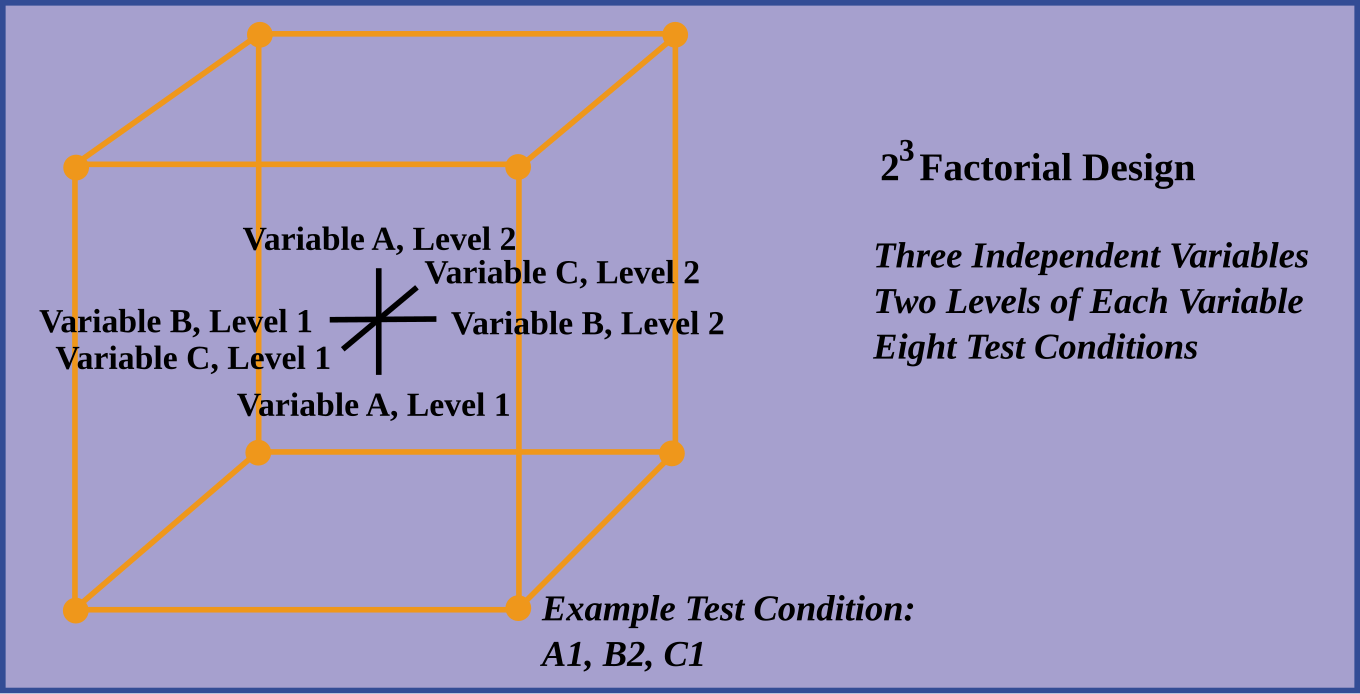
\includegraphics[width=\linewidth]{figures/plano fatorial exemplo}
    \caption{Gráfico de cubos para o plano fatorial.}
    \label{fig:plano_fatorial_exemplo}
\end{marginfigure}

Os planos fatoriais podem ser simplificados se apenas se utilizar dois níveis de variação para cada fator, um nível inferior e um nível superior. 
Por exemplo, um plano fatorial $2\times2$ tem dois fatores, cada um com dois níveis de variação, resultando em quatro combinações únicas que serão testadas.
A interação entre estes fatores é frequentemente o resultado mais importante, mesmo quando os fatores individuais também têm um efeito.

Foram realizados dois planos fatoriais, um plano fatorial para a lixiviação com Tioureia e um plano fatorial para a lixiviação com Citrato.
Para a lixiviação com Tioureia foi elaborado um plano fatorial com 4 fatores\sidenote{Ou seja, 16 combinações, que foram reduzidas a 1/2, resultando em 8 combinações.} e variação de dois níveis.
Para a lixiviação com Citrato foi elaborado um plano fatorial com 6 fatores\sidenote{Ou seja, 64 combinações, que foram reduzidas a 1/8, resultando em 8 combinações.} e variação de dois níveis.

A Tabela~\ref{tab:plano_fatorial_tioureia1} mostra os fatores e os níveis de variação para o plano fatorial com Tioureia.

\begin{table}
  \caption{Fatores e níveis de variação para a Tioureia.}\label{tab:plano_fatorial_tioureia1}
  \begin{tabularx}{\textwidth}{@{}lCC@{}}
    \toprule
    \textbf{Fatores} & \textbf{Nível Inferior} & \textbf{Nível Superior} \\ \midrule
    A - \ce{CH4N2S} (g/kg) & 200 & 300 \\
    B - \ce{Fe(SO4)3} (g/kg) & 1 & 2 \\
    C - Temperatura (\graus{}) & 20 & 60 \\
    D - Tempo (h) & 4 & 6 \\ \bottomrule
  \end{tabularx}
\end{table}

A Tabela~\ref{tab:plano_fatorial_citrato1} mostra os fatores e os níveis de variação para o plano fatorial com Tioureia.

\begin{table}
  \caption{Fatores e níveis de variação para o Citrato.}\label{tab:plano_fatorial_citrato1}
  \begin{tabularx}{\textwidth}{@{}lCC@{}}
    \toprule
    \textbf{Fatores} & \textbf{Nível Inferior} & \textbf{Nível Superior} \\ \midrule
    A - \ce{Na2S2O3} (mol/L) & 0,1 & 0,3 \\
    B - \ce{CuSO4} (mol/L) & 0,1 & 0,2 \\
    C - \ce{Na3C6H5O7} (mol/L) & 0,1 & 0,3 \\
    D - Temperatura (\graus{}) & 50 & 70 \\
    E - Tempo (h) & 7 & 9 \\
    F - pH & 7 & 11 \\ \bottomrule
  \end{tabularx}
\end{table}

Em ambos os planos fatoriais, a quantidade de minério a ser lixiviada e a relação sólido líquido mantiveram-se constantes, sendo 100~g e L/S = 1/5, respetivamente.

\begin{table}
  \caption{Plano fatorial com Tioureia.}
  \begin{tabularx}{\textwidth}{@{}>{\bfseries}CCCCC@{}}
    \toprule
    \textbf{OrdemPad} & \textbf{A} & \textbf{B} & \textbf{C} & \textbf{D} \\ \midrule
    2 & 1 & -1 & -1 & 1 \\
    7 & -1 & 1 & 1 & -1 \\
    4 & 1 & 1 & -1 & -1 \\
    3 & -1 & 1 & -1 & 1 \\
    1 & -1 & -1 & -1 & -1 \\
    8 & 1 & 1 & 1 & 1 \\
    6 & 1 & -1 & 1 & -1 \\
    5 & -1 & -1 & 1 & 1 \\ \bottomrule
  \end{tabularx}
\end{table}

Ou seja, foram realizados 8 ensaios de lixiviação.


\cleardoublepage
\thispagestyle{empty}
% \nocite{*}
\bibliography{main}
\bibliographystyle{plainnat}
%\vspace*{\fill}

\end{document}
